\chapter{Matrices}

\section{Matrices}

\begin{definition}[矩阵]
    \term{矩阵}是一个由数字构成的矩阵数组。 

    \begin{equation} \left[\begin{array}{cccc}0 & 1 & -2.3 & 0.1 \\ 1.3 & 4 & -0.1 & 0 \\ 4.1 & -1 & 0 & 1.7\end{array}\right] \quad  \left(\begin{array}{cccc}0 & 1 & -2.3 & 0.1 \\ 1.3 & 4 & -0.1 & 0 \\ 4.1 & -1 & 0 & 1.7\end{array}\right)  \end{equation}

    上述矩阵\term{大小(size)}为 $3\times 4$, 矩阵的每一个\term{元素(element)}又称为\term{系数(coefficient)};
\end{definition}

\begin{notation}
    设 $ B_{i j} $ 表示矩阵 $ B $ 中第 $ i $ 行第 $ j $列 的元素

    实数域中大小为 $ m \times n $ 的矩阵集合写为 $ \mathfrak{R}^{m \times n} $

    复数域中大小为 $ m \times n $ 的矩阵集合写为 $ \mathbb{C}^{m \times n} $
\end{notation}

\begin{definition}[标量]
    不区分一个$1\times 1$矩阵和一个标量。 
\end{definition}

\begin{definition}[向量]
    不区分一个$n\times 1$矩阵和一个向量。 
\end{definition}

\begin{definition}[行向量, 列向量]
    一个$1\times n$矩阵被称为一个行向量。 
    
    一个$n\times 1$矩阵杯称为一个列向量。 
\end{definition}

\begin{definition}[高形, 宽形和方形矩阵]
    一个大小为$m\times n$的矩阵为:
    \begin{itemize}
        \item \term{高}的, 如果$m>n$
        \item \term{宽}的, 如果$m<n$
        \item \term{方}的, 如果$m=n$
    \end{itemize}
\end{definition}

\begin{definition}[分块矩阵]
    分块矩阵的每一个元素都是一个矩阵。

    \begin{equation} A=\left[\begin{array}{ll}B & C \\ D & E\end{array}\right] \end{equation}

    其中$B,C,D,E$都是矩阵(被称为\term{矩阵$A$的子矩阵}).
\end{definition}

分块矩阵位于同一行的子矩阵行维度必须相等,位于同一列的子矩阵列维度必须相等。

\begin{definition}[矩阵的列向量表示]
    矩阵 $ A \in \mathfrak{R}^{m \times n} $ , 可通过其列向量($m$-vector)进行表示,假设其列向量为 $ a_{1}, \ldots, a_{n} \in \mathfrak{R}^{m} $, 则有

    \begin{equation} A=\left[\begin{array}{lll}a_{1} & \cdots & a_{n}\end{array}\right] \end{equation}
\end{definition}

\begin{definition}[矩阵的行向量表示]
    矩阵 $ A \in \mathfrak{R}^{m \times n} $通过其行向量 $ b_{1}, \ldots, b_{m} $ 进行表示

    \begin{equation} A=\left[\begin{array}{c}b_{1} \\ \vdots \\ b_{m}\end{array}\right], b_{i}^{T} \in \mathfrak{R}^{n}, i=1, \cdots, m \end{equation}
\end{definition}

\section{矩阵运算}

\begin{definition}[矩阵数乘]
    设矩阵 $ A \in \mathfrak{R}^{m \times n} $

    \begin{equation} \beta A=\left[\begin{array}{cccc}\beta A_{11} & \beta A_{12} & \cdots & \beta A_{1 n} \\ \vdots & \vdots & \ddots & \vdots \\ \beta A_{m 1} & \beta A_{m 2} & \cdots & \beta A_{m n}\end{array}\right], \beta \in \mathfrak{R} \end{equation}

    ($ A $ and $ \beta $ can be real or complex.)
\end{definition}

\begin{definition}[矩阵加法]
    矩阵 $ A, B \in \mathfrak{R}^{m \times n} $ 的和为

    \begin{equation} A+B=\left[\begin{array}{cccc}A_{11}+B_{11} & A_{12}+B_{12} & \cdots & A_{1 n}+B_{1 n} \\ \vdots & \vdots & \ddots & \vdots \\ A_{m 1}+B_{m 1} & A_{m 2}+B_{m 2} & \cdots & A_{m n}+B_{m n}\end{array}\right] \end{equation}
\end{definition}

\begin{definition}[Transpose]
    矩阵A的转置表示为 $ A^{T} $
    
    若 $A\in \mathfrak{R}^{m \times n} $, 则 $ A^{T} \in \mathfrak{R}^{n \times m} $ , 其被定义为: $ \left(A^{T}\right)_{i j}=A_{j i}, i=1, \ldots, n ; j=1, \ldots, m $
\end{definition}

转置将原矩阵的行向量转化为列向量。

\begin{corollary}
    [转置的性质]
    有如下性质:
    \begin{itemize}
        \item $ \left(A^{T}\right)^{T}=A $
        \item 对称矩阵满足 $ A^{T}=A $
        \item  $A$ may be complex, but transpose of a complex matrix is rarely needed.
        \item $ (\beta A)^{T}=\beta A^{T},(A+B)^{T}=A^{T}+B^{T} $
    \end{itemize}
\end{corollary}

\begin{definition}[共轭转置]
    矩阵$A$的共轭转置表示为 $ A^{{H}} $
    
    若 $ {A} \in \mathbb{C}^{m \times n} $ , 则 $ A^{H} \in \mathbb{C}^{n \times m} $ , 其被 定义为: $ \left(A^{H}\right)_{i j}=\bar{A}_{j i}, i=1, \ldots, n ; j=1, \ldots, m $;

    设矩阵 $ A \in \mathbb{C}^{m \times n} $ , 则其共轭转置为一个 $ n \times m $ 矩阵

\begin{equation}
A^{H}=\left[\begin{array}{cccc}
\bar{A}_{11} & \bar{A}_{21} & \cdots & \bar{A}_{m 1} \\
\bar{A}_{21} & \bar{A}_{22} & \cdots & \bar{A}_{m 2} \\
\vdots & \vdots & \ddots & \vdots \\
\bar{A}_{1 n} & \bar{A}_{2 n} & \cdots & \bar{A}_{m n}
\end{array}\right]
\end{equation}
\end{definition}

\begin{corollary}[共轭转置的性质]
    有如下性质:
    \begin{itemize}
        \item $ \left(A^{H}\right)^{H}=A $
        \item Hermitian矩阵满足 $ A=A^{H} $
        \item $ (\beta A)^{H}=\beta A^{H},(A+B)^{H}=A^{H}+B^{H} $
    \end{itemize}
\end{corollary}


\begin{definition}[矩阵乘法]
    设矩阵 $ A \in \mathfrak{R}^{m \times p}, B \in \mathfrak{R}^{p \times n} $,那么矩阵$A$与$B$的乘积, 记 作C $ =A B $ ,  矩阵 $ C \in \mathfrak{R}^{m \times n} $ 的第 i行第 $ j $ 列元素 $ C_{i j} $

    \begin{equation}
{C}_{i j}=\sum_{k=1}^{p} A_{i k} B_{k j}
\end{equation}

\end{definition}

\begin{remark}
    矩阵$A$的列大小必须等于$B$的行大小。
\end{remark} 

\begin{corollary}[矩阵乘法性质]
    有如下性质:
    \begin{itemize}
        \item 结合律: $ (A B) C=A(B C) $.
        \item 分配律: $ A(B+C)=A B+A C $.
        \item $ (A B)^{T}=B^{T} A^{T}, \quad(A B)^{{H}}=B^{H} A^{H} $.
        \item 一般情况下 $ A B \neq B A $.
        \item 对于方阵$A$有, $ I A=A I=A $.
    \end{itemize} 
\end{corollary}

\begin{definition}[分块矩阵乘法]
    \begin{equation} \left[\begin{array}{ll}A & B \\ {C} & D\end{array}\right]\left[\begin{array}{ll}W & Y \\ X & Z\end{array}\right]=\left[\begin{array}{ll}A W+B X & A Y+B Z \\ C W+D X & C Y+D Z\end{array}\right] \end{equation}
\end{definition}

\begin{definition}[矩阵-向量乘积 $Ax$]
    矩阵 $ A \in \mathfrak{R}^{m \times n} $ 和一个向量 $ x \in \mathfrak{R}^{n} $ 的积为
\begin{equation}
A x=\left[\begin{array}{c}
A_{11} x_{1}+A_{12} x_{2}+\cdots+A_{1 n} x_{n} \\
A_{21} x_{1}+A_{22} x_{2}+\cdots+A_{2 n} x_{n} \\
\vdots \\
A_{m 1} x_{1}+A_{m 2} x_{2}+\cdots+A_{m n} x_{n}
\end{array}\right]
\end{equation}
\end{definition}

\begin{corollary}
    $ {A} x $ 是矩阵$A$列向量的线性组合。

\begin{equation}
A x=\left[\begin{array}{llll}
a_{1} & a_{2} & \cdots & a_{n}
\end{array}\right]\left[\begin{array}{c}
x_{1} \\
x_{2} \\
\vdots \\
x_{n}
\end{array}\right]=x_{1} a_{1}+\cdots+x_{n} a_{n}
\end{equation}
\end{corollary}

可以引出$A$的Row Picture和Column Picture的概念。

\begin{example}
    \label{exm: row-column-picture}
    \begin{equation}\left\{\begin{matrix} 
        
        x - 2y=1 \\  
        3x+2y=11 
      \end{matrix}\right. \end{equation}




   
\begin{figure}[htbp]
        \caption{Row Picture and Column Picture for \ref{exm: row-column-picture}}
    \begin{subfigure}[b]{0.8\textwidth}
        \centering
        \caption{Row Picture}
    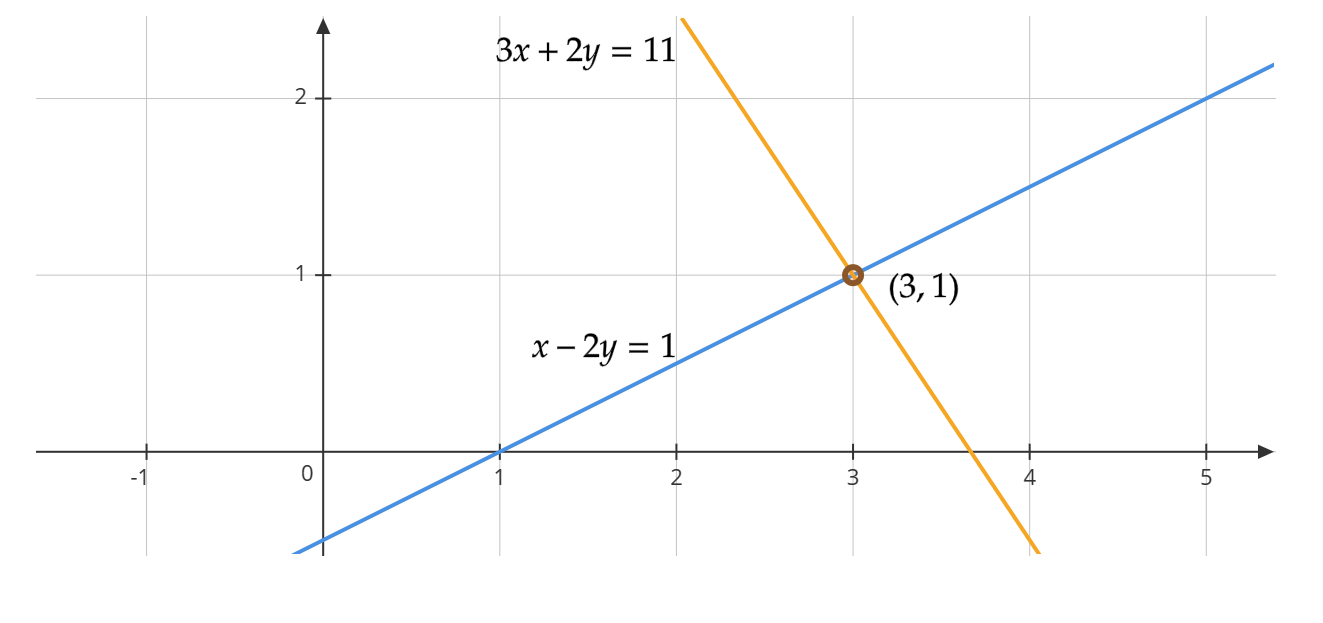
\includegraphics[width=\textwidth]{math-row-picture.png}
    \end{subfigure}

   
    \begin{subfigure}[b]{0.8\textwidth}
        \centering
        \caption{Column Picture}
    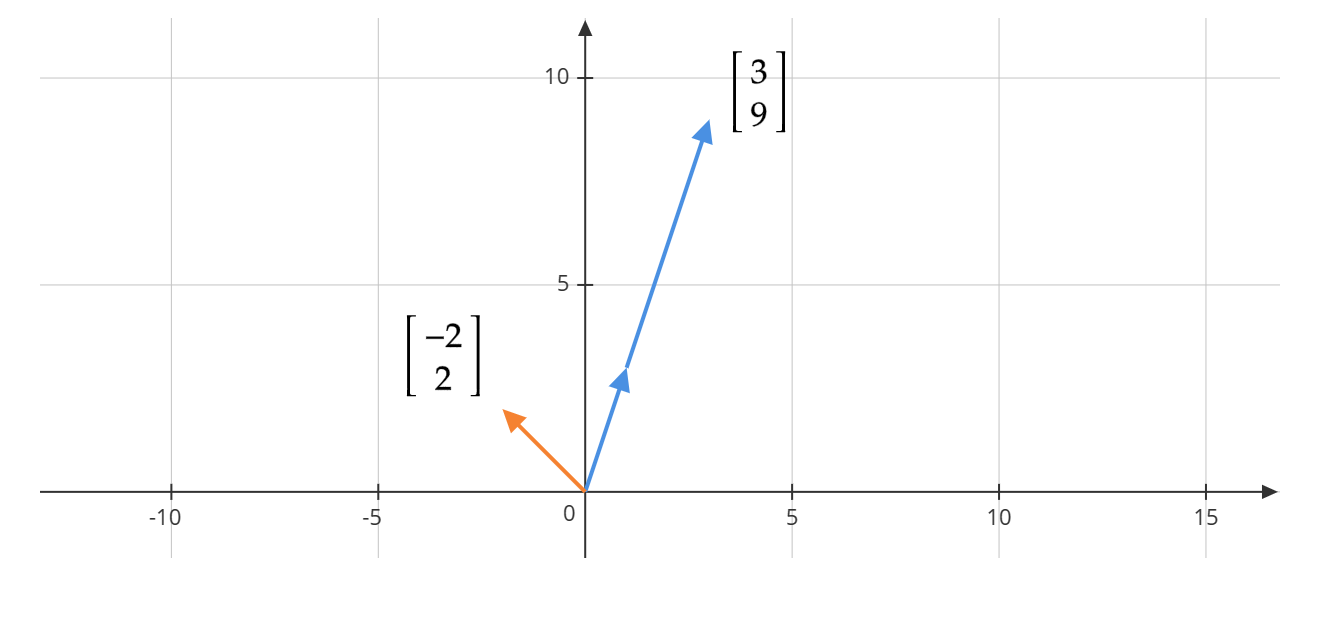
\includegraphics[width=\textwidth]{math-column-picture.png}
    \end{subfigure}
\end{figure}
\end{example}

$ f: \mathfrak{R}^{n} \rightarrow \mathfrak{R}^{m} $ in terms of its effect on $ x $. 

signal processing/control interpretation: $ n $ inputs $ x_{i}, m $ outputs $ y_{i} $. $ f $ is linear if we can represent its action on $ x $ as a product $ f(x)=A x $

\begin{definition}[矩阵-向量乘积函数 $f(x)=A x$]
    给定矩阵 $ A \in \mathfrak{R}^{m \times n} $ , 定义函数 $ f: \mathfrak{R}^{n} \rightarrow \mathfrak{R}^{m}, f(x)=A x $, 其中 $ A=\left[f\left(e_{1}\right) \ldots f\left(e_{n}\right)\right] $.
    
\end{definition}

\begin{theorem}
    矩阵-向量乘积函数$f(x)=A x$为一个线性函数: \begin{equation} A(\alpha x+\beta y)=\alpha(A x)+\beta(A y) \end{equation}
\end{theorem}

\begin{proof}
    
    
    任意一个线性函数都可以写成矩阵-向量乘积函数的形式

    \begin{equation} \begin{aligned} f(x) &=f\left(x_{1} e_{1}+x_{2} e_{2}+\cdots+x_{n} e_{n}\right) \\ &=x_{1} f\left(e_{1}\right)+x_{2} f\left(e_{2}\right)+\cdots+x_{n} f\left(e_{n}\right) \\ &=\left[\begin{array}{lll}f\left(e_{1}\right) & \cdots & f\left(e_{n}\right)\end{array}\right]\left[\begin{array}{c}x_{1} \\ \vdots \\ x_{n}\end{array}\right] \end{aligned} \end{equation}

    因此 $ f(x)=A x $, 其中 $ A=\left[f\left(e_{1}\right) \ldots f\left(e_{n}\right)\right] $
\end{proof}

\subsection{Matrix Power}
It makes sense to multiply a square matrix $ A $ by itself to form $ A A $. 
\begin{definition}[Matrix Power]
    We refer to this matrix as $ A^{2} $. Similarly, if $ k $ is a positive integer, then $ k $ copies of $ A $ multiplied together is denoted $ A^{k} $. 
    
    \begin{equation} \left(A^{\ell+1}\right)_{i j}=\sum_{k=1}^{n} A_{i k}\left(A^{\ell}\right)_{k j} \end{equation}

    By convention we take $ A^{0}=I $, which makes the
    formulas above hold for all nonnegative integer values of $k$ and $l$.
\end{definition}

\begin{theorem}
    If $ k $ and $ l $ are positive integers, and $ A $ is square, then $ A^{k} A^{l}=A^{k+l} $ and $ \left(A^{k}\right)^{l}=A^{k l} $.
\end{theorem}

 \begin{example}[Paths in a directed graph]
        \begin{equation} A_{i j}=\left\{\begin{array}{ll}1 & \text { there is a edge from vertex } j \text { to vertex } i \\ 0 & \text { otherwise }\end{array}\right. \end{equation}
\end{example}

\begin{example}[Linear dynamical system]
    \begin{equation} x_{t+\ell}=A^{\ell} x_{t} \end{equation}
\end{example}

\section{矩阵运算的算法复杂度}

\label{complexity:matrix-operations}

\subsection{矩阵加法、标量数乘、转置、$Ax$的算法复杂度}

The addition of two $ m \times n $ matrices or a scalar multiplication of an $ m \times n $ matrix each take $ m n $ flops.

When $ A $ is sparse, scalar multiplication requires $ \mathbf{n n z}(A) $ flops. 

When at least one of $ A $ and $ B $ is sparse, computing $ A+B $ requires at $ \operatorname{most} \min \{\mathbf{n n z}(A), \mathbf{n n z}(B)\} $ flops. (For any entry $ i, j $ for which one of $ A_{i j} $ or $ B_{i j} $ is zero, no arithmetic operations are needed to find $ \left.(A+B)_{i j} \right) $.

Matrix transposition, i.e., computing $ A^{T} $, requires zero flops, since we simply copy entries of $ A $ to those of $ A^{T} $. (Copying the entries does take time to carry out, but this is not reflected in the flop count.)

A matrix-vector multiplication of an $ m \times n $ matrix $ A $ with an $ n $-vector $ x $ requires $ m(2 n-1) $ flops, which we simplify to $ 2 m n $ flops. This can be seen as follows. The result $ y=A x $ of the product is an $ m $-vector, so there are $ m $ numbers to compute. The $ i $ th element of $ y $ is the inner product of the $ i $ th row of $ A $ and the vector $ x $, which takes $ 2 n-1 $ flops.

If $ A $ is sparse, computing $ A x $ requires $ \mathbf{n n z}(A) $ multiplies (of $ A_{i j} $ and $ x_{j} $, for each nonzero entry of $ A $ ) and a number of additions that is no more than $ \mathbf{n n z}(A) $. Thus, the complexity is between $ \mathbf{n n z}(A) $ and $ 2 \mathbf{n n z}(A) $ flops. As a special example, suppose $ A $ is $ n \times n $ and diagonal. Then $ A x $ can be computed with $ n $ multiplies $ \left(A_{i i}\right. $ times $ x_{i} $ ) and no additions, a total of $ n=\mathbf{n n z}(A) $ flops.

\subsection{矩阵乘法的算法复杂度}

\subsubsection{一般矩阵的乘法}

\begin{theorem}
    Suppose $ C=A B $ with $ A $ of size $ m \times p $ and $ B $ of size $ p \times n $.

    一般矩阵的矩阵乘法的算法复杂度是$O(mnp)$.
\end{theorem}



The product matrix $ C $ has size $ m \times n $, so there are $ m n $ elements to compute. 

The $ i, j $ element of $ C $ is the inner product of row $ i $ of $ A $ with column $ j $ of $ B . $ This is an inner product of vectors of length $ p $ and requires $ 2 p-1 $ flops. Therefore the total is $ m n(2 p-1) $ flops, which we approximate as $ 2 m n p $ flops. 

\subsubsection{稀疏矩阵的乘法}

\begin{theorem}
    Suppose that $ A $ is $ m \times p $ and sparse, and $ B $ is $ p \times n $, but not necessarily sparse. 

    稀疏矩阵乘法的算法复杂度不多于$ 2 \min \{\mathbf{n n z}(A) n, \mathbf{n n z}(B) m\} $ flops.
\end{theorem}



The inner product of the $ i $ th row $ a_{i}^{T} $ of $ A $ with the $ j $ th column of $ B $ requires no more than $ 2 \operatorname{nnz}\left(a_{i}^{T}\right) $ flops. 

Summing over $ i=1, \ldots, m $ and $ j=1, \ldots, n $, we get $ 2 \mathbf{n n z}(A) n $ flops. 

If $ B $ is sparse, the total number of flops is no more that $ 2 \mathbf{n n z}(B) m $ flops. 

There is no simple formula for the complexity of multiplying two sparse matrices, but it is certainly no more than $ 2 \min \{\mathbf{n n z}(A) n, \mathbf{n n z}(B) m\} $ flops.

\begin{remark}
    Note that these formulas agree with the one given above, $ 2 m n p $, when the sparse matrices have all entries nonzero.
\end{remark}

\subsubsection{三重矩阵相乘}

\begin{theorem}
    \begin{equation} D=A B C \end{equation}

with $ A $ of size $ m \times n, B $ of size $ n \times p $, and $ C $ of size $ p \times q $. 

    根据计算顺序的不同,它的算法复杂度是$O( 2 m p(n+q) )$或者$O(2 n q(m+p) )$.
\end{theorem}



The matrix $ D $ can be computed in two ways, as $ (A B) C $ and as $ A(B C) $. 

In the first method we start with $ A B(2 m n p $ flops) and then form $ D=(A B) C(2 m p q $ flops $ ) $, for a total of $ 2 m p(n+q) $ flops. 

In the second method we compute the product $ B C $ (2npq flops) and then form $ D=A(B C)(2 m n q $ flops), for a total of $ 2 n q(m+p) $ flops.

\begin{remark}
    You might guess that the total number of flops required is the same with the two methods, but it turns out it is not. The first method is less expensive when $ 2 m p(n+q)<2 n q(m+p) $, i.e., when
\begin{equation}
\frac{1}{n}+\frac{1}{q}<\frac{1}{m}+\frac{1}{p}
\end{equation}
\end{remark}

\begin{example}
    As a more specific example, consider the product 
    
    \begin{equation} a b^{T} c \end{equation}
    
    where $ a, b, c $ are $ n $ vectors. 
    
    If we first evaluate the outer product $ a b^{T} $, the cost is $ n^{2} $ flops, and we need to store $ n^{2} $ values. We then multiply the vector $ c $ by this $ n \times n $ matrix, which costs $ 2 n^{2} $ flops. The total cost is $ 3 n^{2} $ flops.

    If we first evaluate the inner product $b^Tc$, the cost is $2n$ flops, and we only need to store one number (the result). Multiplying the vector a by this number costs $n$ flops, so the total cost is $3n$ flops. For $n$ large, there is a dramatic difference between $3n$ and $3n^2$ flops.

    (The storage requirements are also dramatically different for the two methods of evaluating $ab^Tc$: $1$ number versus $n^2$ numbers.)
\end{example}

\subsection{矩阵向量乘积复杂度}

矩阵 $ A \in \mathfrak{R}^{m \times n} $ 和向量 $ x \in \mathfrak{R}^{n} $ 的乘积 $ {y}={A} x $, 需要 $ (2 {n}-1) {m} $ flops;

乘积 $ y \in \mathfrak{R}^{m} $ , 每个元素需要做向量内积, 需要 $ 2 n-1 $ flops;

当$n$足够大时, 复杂度近似于$2mn$;

特殊情况:

\begin{itemize}
    \item $A$为对角矩阵: $ {n} $ flops
    \item $A$为下三角矩阵: $ n^{2} $ flops
    \item $A$为稀疏矩阵时:flops $ <<2 m n $
\end{itemize}


\section{Special Matrices and Matrices in Different Applications}

\begin{definition}[Zero Matrix]
    所有元素都为0的矩阵。

    记作\begin{equation}0, 0_{m \times n} \end{equation}
\end{definition}

\begin{definition}[单位矩阵]
    为方形矩阵, 其中对角线元素为1, 其它元素为0.

    记作$I$或者 $ {I}_{n} $.
\end{definition}

\begin{corollary}
  $ {I}_{n} $ 的每一列是一个单位向量, 例如

\begin{equation}
{I}_{3}=\left[\begin{array}{lll}
1 & 0 & 0 \\
0 & 1 & 0 \\
0 & 0 & 1
\end{array}\right]=\left[\begin{array}{lll}
e_{1} & e_{2} & e_{3}
\end{array}\right]
\end{equation}
\end{corollary}

\begin{definition}[Symmetric Matrices]
    \begin{equation} A_{i j}=A_{j i}, A^T =A \end{equation}
\end{definition}

\begin{definition}[Hermitian Matrices]
    $ A_{i j}=\bar{A}_{j i}, A^H = A $ (共轭复数).
\end{definition}

\begin{remark}
    diagonal elements are real (since $ A_{i i}=\bar{A}_{i i} $ ).
\end{remark}

\begin{definition}[Diagonal Matrices]
    对角线上元素不全为0, 其余元素全为0.
\end{definition}

对角矩阵用于膨胀 (dilation).

\begin{definition}[下三角矩阵]
    方形矩阵且当 $ i<j $ 时 $ A_{i j}=0 $.
\end{definition}

\begin{definition}[上三角矩阵]
    方形矩阵且当 $ i>j $ 时 $ A_{i j}=0 $
\end{definition}

通过Gram-Schmidt正交化算法可以化为上三角或者下三角矩阵。

\begin{definition}[Sparse Matrices]
    a matrix is sparse if most (almost all) of its elements are zero
\end{definition}

sparse matrix storage formats and algorithms exploit sparsity, efficiency depends on number of nonzeros and their positions. The positions of nonzeros are visualized in a `spy plot'.

\subsection{$f(x)=A x$中的$A$ (几何变换)}

引入上节$f(x)=A x$(矩阵-向量乘积函数)的概念,

\begin{definition}[Scaling]
    Scaling is the mapping $ y=a x $, where $ a $ is a scalar. This can be expressed as $ y=A x $ with $ A=a I $. This mapping stretches a vector by the factor $ |a| $ (or shrinks it when $ |a|<1 $ ), and it flips the vector (reverses its direction) if $ a<0 $.
\end{definition}

\begin{definition}[Dilation]
    Dilation is the mapping $ y=D x $, where $ D $ is a diagonal matrix, $ D= $ $ \operatorname{diag}\left(d_{1}, d_{2}\right) $. This mapping stretches the vector $ x $ by different factors along the two different axes. (Or shrinks, if $ \left|d_{i}\right|<1 $, and flips, if $ d_{i}<0 $.)
\end{definition}







\begin{definition}[旋转矩阵]
    \begin{equation} A=\left[\begin{array}{cc}\cos \theta & -\sin \theta \\ \sin \theta & \cos \theta\end{array}\right] \end{equation}

    $ {A} x $ 将向量 $ x $ 进行旋转, 角度为 $ \theta $.
\end{definition}

\begin{definition}[Reflection Matrices]
    Suppose that $y$ is the vector obtained by reflecting $x$ through the line
    that passes through the origin, inclined $\theta$ radians with respect to horizontal. Then

    \begin{equation} y=\left[\begin{array}{rr}\cos (2 \theta) & \sin (2 \theta) \\ \sin (2 \theta) & -\cos (2 \theta)\end{array}\right] x \end{equation}
\end{definition}


\begin{definition}[Projection onto a Line]
    The projection of the point $ x $ onto a set is the point in the set that is closest to $ x $. Suppose $ y $ is the projection of $ x $ onto the line that passes through the origin, inclined $ \theta $ radians with respect to horizontal. Then we have
\begin{equation}
y=\left[\begin{array}{cc}
(1 / 2)(1+\cos (2 \theta)) & (1 / 2) \sin (2 \theta) \\
(1 / 2) \sin (2 \theta) & (1 / 2)(1-\cos (2 \theta))
\end{array}\right] x .
\end{equation}
\end{definition}

% todo (2021-12-31 09:47): 149

\subsection{Finding the Geometric Transformation Matrix}

When a geometric transformation is represented by matrix-vector multiplication (as in the examples above), a simple method to find the matrix is to find its columns. \textbf{The $ i $ th column is the vector obtained by applying the transformation to $ e_{i} . $}

\begin{example}
    As a simple example consider clockwise rotation by $ 90^{\circ} $ in 2-D. Rotating the vector $ e_{1}=(1,0) $ by $ 90^{\circ} $ gives $ (0,-1) $; rotating $ e_{2}=(0,1) $ by $ 90^{\circ} $ gives $ (1,0) $. So rotation by $ 90^{\circ} $ is given by
\begin{equation}
y=\left[\begin{array}{rr}
0 & 1 \\
-1 & 0
\end{array}\right] x .
\end{equation}
\end{example}

\begin{example}[Changeof Coordinates]
    Change of coordinates. In many applications multiple coordinate systems are used to describe locations or positions in 2-D or 3-D. For example in aerospace engineering we can describe a position using earth-fixed coordinates or body-fixed coordinates, where the body refers to an aircraft. Earth-fixed coordinates are with respect to a specific origin, with the three axes pointing East, North, and straight up, respectively. The origin of the body-fixed coordinates is a specific location on the aircraft (typically the center of gravity), and the three axes point forward (along the aircraft body), left (with respect to the aircraft body), and up (with respect to the aircraft body). Suppose the 3 -vector $ x^{\text {body }} $ describes a location using the body coordinates, and $ x^{\text {earth }} $ describes the same location in earth-fixed coordinates. These are related by
\begin{equation}
x^{\text {earth }}=p+Q x^{\text {body }},
\end{equation}

where $ p $ is the location of the airplane center (in earth-fixed coordinates) and $ Q $ is a $ 3 \times 3 $ matrix. The $ i $ th column of $ Q $ gives the earth-fixed coordinates for the $ i $ th
axis of the airplane. For an airplane in level flight, heading due South, we have
\begin{equation}
Q=\left[\begin{array}{rrr}
0 & 1 & 0 \\
-1 & 0 & 0 \\
0 & 0 & 1
\end{array}\right]
\end{equation}
\end{example}


\subsection{$f(x)=A x$中的$A$(其他例子)}

\begin{example}[Negation]
    $ f $ changes the sign of $ x: f(x)=-x $.

Negation can be expressed as $ f(x)=A x $ with $ A=-I $.
\end{example}

\begin{example}[Running Sum Matrix]
    The $ n \times n $ matrix
\begin{equation}
S=\left[\begin{array}{cccccc}
1 & 0 & 0 & \ldots & 0 & 0 \\
1 & 1 & 0 & \ldots & 0 & 0 \\
& & \ddots & \ddots & & \\
& & & \ddots & \ddots & \\
1 & 1 & 1 & \ldots & 1 & 0 \\
1 & 1 & 1 & \ldots & 1 & 1
\end{array}\right]
\end{equation}
is called the running sum matrix. 

The $ i $ th entry of the $ n $-vector $ S x $ is the sum of the first $ i $ entries of $ x $ :
\begin{equation}
S x=\left[\begin{array}{c}
x_{1} \\
x_{1}+x_{2} \\
x_{1}+x_{2}+x_{3} \\
\vdots \\
x_{1}+\cdots+x_{n}
\end{array}\right]
\end{equation}
\end{example}

\begin{example}[De-meaning, Centering Matrix]
    $ f $ subtracts the mean from each entry of a vector $ x $ : $ f(x)= $ $ x-\operatorname{avg}(x) $ 1.

The de-meaning function can be expressed as $ f(x)=A x $ with
\begin{equation}
A=\left[\begin{array}{cccc}
1-1 / n & -1 / n & \cdots & -1 / n \\
-1 / n & 1-1 / n & \cdots & -1 / n \\
\vdots & \vdots & \ddots & \vdots \\
-1 / n & -1 / n & \cdots & 1-1 / n
\end{array}\right] \text {. }
\end{equation}
\end{example}

\begin{example}
    $ f $ 对向量 $ x $ 中的元素进行升序排序, 非线性;
\end{example}

\begin{example}
    $ f $ 将向量 $ x $ 中的元素替换成相应的绝对值, 非线性;
\end{example}


\subsection{Selectors}



\begin{definition}[Selector matrices]
    An $ m \times n $ selector matrix $ A $ is one in which each row is a unit vector (transposed)
\begin{equation}
A=\left[\begin{array}{c}
e_{k_{1}}^{T} \\
\vdots \\
e_{k_{m}}^{T}
\end{array}\right]
\end{equation}
where $ k_{1}, \ldots, k_{m} $ are integers in the range $ 1, \ldots, n . $ 
\end{definition}

When it multiplies a vector, it simply copies the $ k_{i} $ th entry of $ x $ into the $ i $ th entry of $ y=A x $ :
\begin{equation}
y=\left(x_{k_{1}}, x_{k_{2}}, \ldots, x_{k_{m}}\right) .
\end{equation}

In words, each entry of $ A x $ is a selection of an entry of $ x $.

The identity matrix, and the reverser matrix are special cases of selector matrices.

\begin{definition}[Permutation Matrices]
    $ f $ 颠倒向量 $ x $ 中的元素的顺序, 一个线性函数 $ f(x)=A x $

    \begin{equation} A=\left[\begin{array}{lll}0 & 0 & 1 \\ 0 & 1 & 0 \\ 1 & 0 & 0\end{array}\right] \end{equation}是一个置换矩阵。
\end{definition}

\begin{proof}
    \begin{equation} A x=\left[\begin{array}{lll}0 & 0 & 1 \\ 0 & 1 & 0 \\ 1 & 0 & 0\end{array}\right]\left[\begin{array}{l}x_{1} \\ x_{2} \\ x_{3}\end{array}\right]=\left[\begin{array}{l}x_{3} \\ x_{2} \\ x_{1}\end{array}\right] \end{equation}
\end{proof}

\begin{definition}[反转矩阵(Reverser matrix)]
    \begin{equation} A=\left[\begin{array}{ccccc}0 & 0 & \cdots & 0 & 1 \\ 0 & 0 & \cdots & 1 & 0 \\ \vdots & \vdots & \therefore & \vdots & \vdots \\ 0 & 1 & \cdots & 0 & 0 \\ 1 & 0 & \cdots & 0 & 0\end{array}\right] \end{equation}
\end{definition}

\begin{proof}
    \begin{equation} A x=\left[\begin{array}{c}x_{n} \\ x_{n-1} \\ \vdots \\ x_{2} \\ x_{1}\end{array}\right] \end{equation}
\end{proof}

\begin{definition}[循环移位矩阵(Circular shift matrix)]
    \begin{equation} A=\left[\begin{array}{ccccc}0 & 0 & \cdots & 0 & 1 \\ 1 & 0 & \cdots & 0 & 0 \\ 0 & 1 & \cdots & 0 & 0 \\ \vdots & \vdots & \ddots & \vdots & \vdots \\ 0 & 0 & \cdots & 1 & 0\end{array}\right] \end{equation}
\end{definition}

\begin{proof}
    \begin{equation} A x=\left[\begin{array}{c}x_{n} \\ x_{1} \\ x_{2} \\ \vdots \\ x_{n-1}\end{array}\right] \end{equation}
\end{proof}

\begin{definition}[Downsampling]
    Down-sampling. Another example is the $ (n / 2) \times n $ matrix (with $ n $ even)
\begin{equation}
A=\left[\begin{array}{ccccccccccc}
1 & 0 & 0 & 0 & 0 & 0 & \cdots & 0 & 0 & 0 & 0 \\
0 & 0 & 1 & 0 & 0 & 0 & \cdots & 0 & 0 & 0 & 0 \\
0 & 0 & 0 & 0 & 1 & 0 & \cdots & 0 & 0 & 0 & 0 \\
\vdots & \vdots & \vdots & \vdots & \vdots & \vdots & & \vdots & \vdots & \vdots & \vdots \\
0 & 0 & 0 & 0 & 0 & 0 & \cdots & 1 & 0 & 0 & 0 \\
0 & 0 & 0 & 0 & 0 & 0 & \cdots & 0 & 0 & 1 & 0
\end{array}\right] \text {. }
\end{equation}
\end{definition}

\begin{example}
    If $ y=A x $, we have $ y=\left(x_{1}, x_{3}, x_{5}, \ldots, x_{n-3}, x_{n-1}\right) $. When $ x $ is a time series, $ y $ is called the $ 2 \times $ down-sampled version of $ x $.
\end{example}

\subsection{图论中的矩阵}


\begin{definition}[关联矩阵]
   假设有向图$G$有$m$个顶点,  $ n $ 条弧, 则关联矩阵$A$大小为 $ m \times n $,其中 

   \begin{equation} A_{i j}=\left\{\begin{array}{ll}1 & \text{如果点} i \text{是弧} j \text{的终点 } \\ -1 & \text {如果点}i \text{是弧}j \text{的起点} \\ 0 & \text { 其它 }\end{array}\right. \end{equation}
\end{definition}

\begin{example}[路径矩阵]
\begin{FigureCenter}{Paths in Directed Graph}
\tikzset{every picture/.style={line width=0.75pt}} %set default line width to 0.75pt        

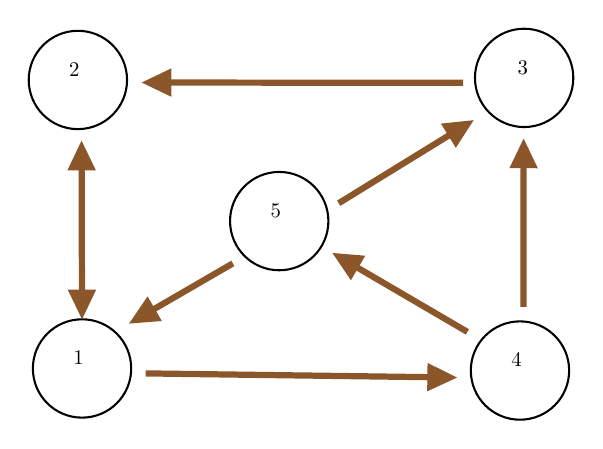
\begin{tikzpicture}[x=0.75pt,y=0.75pt,yscale=-1,xscale=1]
%uncomment if require: \path (0,300); %set diagram left start at 0, and has height of 300

%Shape: Circle [id:dp5532284801725602] 
\draw   (213.62,88.69) .. controls (213.62,75.61) and (224.22,65) .. (237.31,65) .. controls (250.39,65) and (261,75.61) .. (261,88.69) .. controls (261,101.78) and (250.39,112.38) .. (237.31,112.38) .. controls (224.22,112.38) and (213.62,101.78) .. (213.62,88.69) -- cycle ;
%Shape: Circle [id:dp7238339296497196] 
\draw   (428.62,87.69) .. controls (428.62,74.61) and (439.22,64) .. (452.31,64) .. controls (465.39,64) and (476,74.61) .. (476,87.69) .. controls (476,100.78) and (465.39,111.38) .. (452.31,111.38) .. controls (439.22,111.38) and (428.62,100.78) .. (428.62,87.69) -- cycle ;
%Shape: Circle [id:dp9299746230640014] 
\draw   (310.62,156.69) .. controls (310.62,143.61) and (321.22,133) .. (334.31,133) .. controls (347.39,133) and (358,143.61) .. (358,156.69) .. controls (358,169.78) and (347.39,180.38) .. (334.31,180.38) .. controls (321.22,180.38) and (310.62,169.78) .. (310.62,156.69) -- cycle ;
%Shape: Circle [id:dp06003655838365507] 
\draw   (215.62,227.69) .. controls (215.62,214.61) and (226.22,204) .. (239.31,204) .. controls (252.39,204) and (263,214.61) .. (263,227.69) .. controls (263,240.78) and (252.39,251.38) .. (239.31,251.38) .. controls (226.22,251.38) and (215.62,240.78) .. (215.62,227.69) -- cycle ;
%Shape: Circle [id:dp9333980197615774] 
\draw   (426.62,228.69) .. controls (426.62,215.61) and (437.22,205) .. (450.31,205) .. controls (463.39,205) and (474,215.61) .. (474,228.69) .. controls (474,241.78) and (463.39,252.38) .. (450.31,252.38) .. controls (437.22,252.38) and (426.62,241.78) .. (426.62,228.69) -- cycle ;
%Straight Lines [id:da14351861661944953] 
\draw [color={rgb, 255:red, 139; green, 87; blue, 42 }  ,draw opacity=1 ][line width=2.25]    (239.29,199) -- (239.09,122.93) ;
\draw [shift={(239.07,117.93)}, rotate = 89.84] [fill={rgb, 255:red, 139; green, 87; blue, 42 }  ,fill opacity=1 ][line width=0.08]  [draw opacity=0] (14.29,-6.86) -- (0,0) -- (14.29,6.86) -- cycle    ;
\draw [shift={(239.31,204)}, rotate = 269.84] [fill={rgb, 255:red, 139; green, 87; blue, 42 }  ,fill opacity=1 ][line width=0.08]  [draw opacity=0] (14.29,-6.86) -- (0,0) -- (14.29,6.86) -- cycle    ;
%Straight Lines [id:da17800771926651127] 
\draw [color={rgb, 255:red, 139; green, 87; blue, 42 }  ,draw opacity=1 ][line width=2.25]    (422.97,90.07) -- (273.07,89.93) ;
\draw [shift={(268.07,89.93)}, rotate = 0.05] [fill={rgb, 255:red, 139; green, 87; blue, 42 }  ,fill opacity=1 ][line width=0.08]  [draw opacity=0] (14.29,-6.86) -- (0,0) -- (14.29,6.86) -- cycle    ;
%Straight Lines [id:da8693343970271716] 
\draw [color={rgb, 255:red, 139; green, 87; blue, 42 }  ,draw opacity=1 ][line width=2.25]    (451.97,198.07) -- (452.07,121.93) ;
\draw [shift={(452.07,116.93)}, rotate = 90.07] [fill={rgb, 255:red, 139; green, 87; blue, 42 }  ,fill opacity=1 ][line width=0.08]  [draw opacity=0] (14.29,-6.86) -- (0,0) -- (14.29,6.86) -- cycle    ;
%Straight Lines [id:da6344324541430564] 
\draw [color={rgb, 255:red, 139; green, 87; blue, 42 }  ,draw opacity=1 ][line width=2.25]    (269.97,230.07) -- (414.97,232) ;
\draw [shift={(419.97,232.07)}, rotate = 180.76] [fill={rgb, 255:red, 139; green, 87; blue, 42 }  ,fill opacity=1 ][line width=0.08]  [draw opacity=0] (14.29,-6.86) -- (0,0) -- (14.29,6.86) -- cycle    ;
%Straight Lines [id:da07777304568721788] 
\draw [color={rgb, 255:red, 139; green, 87; blue, 42 }  ,draw opacity=1 ][line width=2.25]    (424.97,210.07) -- (364.28,174.59) ;
\draw [shift={(359.97,172.07)}, rotate = 30.31] [fill={rgb, 255:red, 139; green, 87; blue, 42 }  ,fill opacity=1 ][line width=0.08]  [draw opacity=0] (14.29,-6.86) -- (0,0) -- (14.29,6.86) -- cycle    ;
%Straight Lines [id:da043097960393339685] 
\draw [color={rgb, 255:red, 139; green, 87; blue, 42 }  ,draw opacity=1 ][line width=2.25]    (362.97,148.07) -- (423.71,110.69) ;
\draw [shift={(427.97,108.07)}, rotate = 148.39] [fill={rgb, 255:red, 139; green, 87; blue, 42 }  ,fill opacity=1 ][line width=0.08]  [draw opacity=0] (14.29,-6.86) -- (0,0) -- (14.29,6.86) -- cycle    ;
%Straight Lines [id:da4103672479327105] 
\draw [color={rgb, 255:red, 139; green, 87; blue, 42 }  ,draw opacity=1 ][line width=2.25]    (311.97,177.07) -- (266.29,203.56) ;
\draw [shift={(261.97,206.07)}, rotate = 329.89] [fill={rgb, 255:red, 139; green, 87; blue, 42 }  ,fill opacity=1 ][line width=0.08]  [draw opacity=0] (14.29,-6.86) -- (0,0) -- (14.29,6.86) -- cycle    ;

% Text Node
\draw (232,79.4) node [anchor=north west][inner sep=0.75pt]  [xscale=0.75,yscale=0.75]  {$2$};
% Text Node
\draw (448,78.4) node [anchor=north west][inner sep=0.75pt]  [xscale=0.75,yscale=0.75]  {$3$};
% Text Node
\draw (329,147.4) node [anchor=north west][inner sep=0.75pt]  [xscale=0.75,yscale=0.75]  {$5$};
% Text Node
\draw (234,218.4) node [anchor=north west][inner sep=0.75pt]  [xscale=0.75,yscale=0.75]  {$1$};
% Text Node
\draw (445,219.4) node [anchor=north west][inner sep=0.75pt]  [xscale=0.75,yscale=0.75]  {$4$};


\end{tikzpicture}
\end{FigureCenter}


    matrix representation
\begin{equation}
A=\left[\begin{array}{lllll}
0 & 1 & 0 & 0 & 1 \\
1 & 0 & 1 & 0 & 0 \\
0 & 0 & 0 & 1 & 1 \\
1 & 0 & 0 & 0 & 0 \\
0 & 0 & 0 & 1 & 0
\end{array}\right]
\end{equation}
$ A_{i j}=1 $ indicates an edge $ j \rightarrow i $

    give a graph interpretation of $ A^{2}=A A, A^{3}=A A A, \ldots $
\begin{equation}
A^{2}=\left[\begin{array}{lllll}
1 & 0 & 1 & 1 & 0 \\
0 & 1 & 0 & 1 & 2 \\
1 & 0 & 0 & 1 & 0 \\
0 & 1 & 0 & 0 & 1 \\
1 & 0 & 0 & 0 & 0
\end{array}\right], \quad A^{3}=\left[\begin{array}{lllll}
1 & 1 & 0 & 1 & 2 \\
2 & 0 & 1 & 2 & 0 \\
1 & 1 & 0 & 0 & 1 \\
1 & 0 & 1 & 1 & 0 \\
0 & 1 & 0 & 0 & 1
\end{array}\right]
\end{equation}
\end{example}


\subsection{网络中的矩阵}

In many applications a graph is used to represent a network, through which some commodity or quantity such as electricity, water, heat, or vehicular traffic flows. The edges of the graph represent the paths or links over which the quantity can move or flow, in either direction. If $ x $ is an $ m $-vector representing a flow in the network, we interpret $ x_{j} $ as the flow (rate) along the edge $ j $, with a positive value meaning the flow is in the direction of edge $ j $, and negative meaning the flow is in the opposite direction of edge $ j $. In a network, the direction of the edge or link does not specify the direction of flow; it only specifies which direction of flow we consider to be positive.

\subsubsection{Flow conservation}

When $ x $ represents a flow in a network, the matrix-vector product $ y=A x $ can be given a very simple interpretation. 

The $ n $-vector $ y=A x $ can be interpreted as the vector of net flows, from the edges, into the nodes: $ y_{i} $ is equal to the total of the flows that come in to node $ i $, minus the total of the flows that go out from node $ i $. The quantity $ y_{i} $ is sometimes called the \term{flow surplus} at node $ i $.

If $ A x=0 $, we say that \term{flow conservation} occurs, since at each node, the total inflow matches the total out-flow. In this case the flow vector $ x $ is called a \term{circulation}. This could be used as a model of traffic flow (in a closed system), with the nodes representing intersections and the edges representing road segments (one for each
direction).

\subsubsection{Sources and Sinks}

In many applications it is useful to include additional flows called \term{source flows} or \term{exogenous flows}, that enter or leave the network at the nodes, but not along the edges. We denote these flows with an $ n $-vector $ s $. 

We can think of $ s_{i} $ as a flow that enters the network at node $ i $ from outside, i.e., not from any edge. When $ s_{i}>0 $ the exogenous flow is called a \term{source}, since it is injecting the quantity into the network at the node. When $ s_{i}<0 $ the exogenous flow is called a \term{sink}, since it is removing the quantity from the network at the node.

\subsubsection{Flow Conservation with Sources}

The equation $Ax + s = 0$ means that the flow
is conserved at each node, counting the source flow: The total of all incoming flow,
from the incoming edges and exogenous source, minus the total outgoing flow from
outgoing edges and exogenous sinks, is zero.

\subsubsection{Node Potentials}

A graph is also useful when we focus on the values of some quantity at each graph vertex or node. Let $ v $ be an $ n $-vector, often interpreted as a potential, with $ v_{i} $ the potential value at node $ i $. We can give a simple interpretation to the matrix-vector product $ u=A^{T} v $. The $ m $-vector $ u=A^{T} v $ gives the potential differences across the edges: $ u_{j}=v_{l}-v_{k} $, where edge $ j $ goes from node $ k $ to node $ l $.

\subsubsection{Dirichlet Energy}

When the $ m $-vector $ A^{T} v $ is small, it means that the potential differences across the edges are small. Another way to say this is that the potentials of connected vertices are near each other. A quantitative measure of this is the function of $ v $ given by
\begin{equation}
\mathcal{D}(v)=\left\|A^{T} v\right\|^{2}
\end{equation}
This function arises in many applications, and is called the Dirichlet energy (or Laplacian quadratic form) associated with the graph. It can be expressed as
\begin{equation}
\mathcal{D}(v)=\sum_{\text {edges }(k, l)}\left(v_{l}-v_{k}\right)^{2}
\end{equation}

which is the sum of the squares of the potential differences of v across all edges in
the graph. The Dirichlet energy is small when the potential differences across the
edges of the graph are small, i.e., nodes that are connected by edges have similar
potential values.
The Dirichlet energy is used as a measure the non-smoothness (roughness) of
a set of node potentials on a graph. A set of node potentials with small Dirichlet
energy can be thought of as smoothly varying across the graph. Conversely, a set
of potentials with large Dirichlet energy can be thought of as non-smooth or rough.
The Dirichlet energy will arise as a measure of roughness in several applications.

\subsection{Convolution}


\begin{definition}[一维卷积]
    向量 $ a \in \mathfrak{R}^{n} $ 和向量 $ b \in \mathfrak{R}^{m} $ 的\term{卷积}是一个 $ ({n}+{m}-1) $ 维向量 $ c \in \mathfrak{R}^{m+{n}-1} $

    \begin{equation} c_{k}=\sum_{i+j=k+1} a_{i} b_{j}, \quad k=1, \ldots n+m-1 \end{equation}

    记为 $ c=a * b$
\end{definition}

\begin{example}
    设$n=4,  m=3 $

\begin{FigureCenter}{An Example of Convolution}
    \tikzset{every picture/.style={line width=0.75pt}} %set default line width to 0.75pt        

    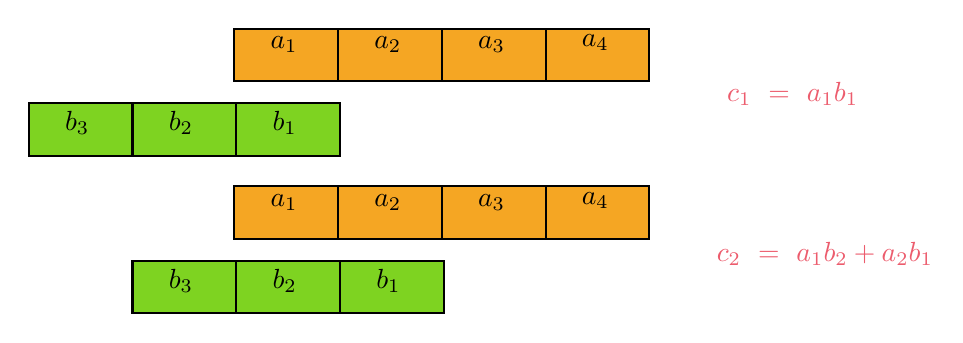
\begin{tikzpicture}[x=0.75pt,y=0.75pt,yscale=-1,xscale=1]
    %uncomment if require: \path (0,300); %set diagram left start at 0, and has height of 300
    
    %Shape: Rectangle [id:dp6383640467867335] 
    \draw  [fill={rgb, 255:red, 245; green, 166; blue, 35 }  ,fill opacity=1 ] (110,54) -- (160.01,54) -- (160.01,79.16) -- (110,79.16) -- cycle ;
    
    %Shape: Rectangle [id:dp9915913508162717] 
    \draw  [fill={rgb, 255:red, 245; green, 166; blue, 35 }  ,fill opacity=1 ] (260.01,54) -- (310.02,54) -- (310.02,79.16) -- (260.01,79.16) -- cycle ;
    %Shape: Rectangle [id:dp7574544776550791] 
    \draw  [fill={rgb, 255:red, 245; green, 166; blue, 35 }  ,fill opacity=1 ] (210,54) -- (260.01,54) -- (260.01,79.16) -- (210,79.16) -- cycle ;
    %Shape: Rectangle [id:dp15668905720803483] 
    \draw  [fill={rgb, 255:red, 245; green, 166; blue, 35 }  ,fill opacity=1 ] (160,54) -- (210.01,54) -- (210.01,79.16) -- (160,79.16) -- cycle ;
    
    %Shape: Rectangle [id:dp517800094810728] 
    \draw  [fill={rgb, 255:red, 126; green, 211; blue, 33 }  ,fill opacity=1 ] (11,90) -- (61.01,90) -- (61.01,115.16) -- (11,115.16) -- cycle ;
    %Shape: Rectangle [id:dp15583903887589012] 
    \draw  [fill={rgb, 255:red, 126; green, 211; blue, 33 }  ,fill opacity=1 ] (61,90) -- (111.01,90) -- (111.01,115.16) -- (61,115.16) -- cycle ;
    %Shape: Rectangle [id:dp4794201673076599] 
    \draw  [fill={rgb, 255:red, 126; green, 211; blue, 33 }  ,fill opacity=1 ] (111,90) -- (161.01,90) -- (161.01,115.16) -- (111,115.16) -- cycle ;
    
    %Shape: Rectangle [id:dp9652913856506695] 
    \draw  [fill={rgb, 255:red, 245; green, 166; blue, 35 }  ,fill opacity=1 ] (110,130) -- (160.01,130) -- (160.01,155.16) -- (110,155.16) -- cycle ;
    
    %Shape: Rectangle [id:dp6681556567962323] 
    \draw  [fill={rgb, 255:red, 245; green, 166; blue, 35 }  ,fill opacity=1 ] (260.01,130) -- (310.02,130) -- (310.02,155.16) -- (260.01,155.16) -- cycle ;
    %Shape: Rectangle [id:dp0819288495364412] 
    \draw  [fill={rgb, 255:red, 245; green, 166; blue, 35 }  ,fill opacity=1 ] (210,130) -- (260.01,130) -- (260.01,155.16) -- (210,155.16) -- cycle ;
    %Shape: Rectangle [id:dp015621153657017217] 
    \draw  [fill={rgb, 255:red, 245; green, 166; blue, 35 }  ,fill opacity=1 ] (160,130) -- (210.01,130) -- (210.01,155.16) -- (160,155.16) -- cycle ;
    
    %Shape: Rectangle [id:dp9772799588063847] 
    \draw  [fill={rgb, 255:red, 126; green, 211; blue, 33 }  ,fill opacity=1 ] (61,166) -- (111.01,166) -- (111.01,191.16) -- (61,191.16) -- cycle ;
    %Shape: Rectangle [id:dp8281584537494973] 
    \draw  [fill={rgb, 255:red, 126; green, 211; blue, 33 }  ,fill opacity=1 ] (111,166) -- (161.01,166) -- (161.01,191.16) -- (111,191.16) -- cycle ;
    %Shape: Rectangle [id:dp20253755057026024] 
    \draw  [fill={rgb, 255:red, 126; green, 211; blue, 33 }  ,fill opacity=1 ] (161,166) -- (211.01,166) -- (211.01,191.16) -- (161,191.16) -- cycle ;
    
    
    % Text Node
    \draw (126,56.4) node [anchor=north west][inner sep=0.75pt]    {$a_{1}$};
    % Text Node
    \draw (176,56.4) node [anchor=north west][inner sep=0.75pt]    {$a_{2}$};
    % Text Node
    \draw (226,56.4) node [anchor=north west][inner sep=0.75pt]    {$a_{3}$};
    % Text Node
    \draw (276,55.4) node [anchor=north west][inner sep=0.75pt]    {$a_{4}$};
    % Text Node
    \draw (127,92.4) node [anchor=north west][inner sep=0.75pt]    {$b_{1}$};
    % Text Node
    \draw (77,92.4) node [anchor=north west][inner sep=0.75pt]    {$b_{2}$};
    % Text Node
    \draw (27,92.4) node [anchor=north west][inner sep=0.75pt]    {$b_{3}$};
    % Text Node
    \draw (77,168.4) node [anchor=north west][inner sep=0.75pt]    {$b_{3}$};
    % Text Node
    \draw (127,168.4) node [anchor=north west][inner sep=0.75pt]    {$b_{2}$};
    % Text Node
    \draw (177,168.4) node [anchor=north west][inner sep=0.75pt]    {$b_{1}$};
    % Text Node
    \draw (276,131.4) node [anchor=north west][inner sep=0.75pt]    {$a_{4}$};
    % Text Node
    \draw (226,132.4) node [anchor=north west][inner sep=0.75pt]    {$a_{3}$};
    % Text Node
    \draw (176,132.4) node [anchor=north west][inner sep=0.75pt]    {$a_{2}$};
    % Text Node
    \draw (126,132.4) node [anchor=north west][inner sep=0.75pt]    {$a_{1}$};
    % Text Node
    \draw (346,78.4) node [anchor=north west][inner sep=0.75pt]  [color={rgb, 255:red, 236; green, 92; blue, 109 }  ,opacity=1 ]  {$c_{1} \ =\ a_{1} b_{1}$};
    % Text Node
    \draw (341,155.4) node [anchor=north west][inner sep=0.75pt]  [color={rgb, 255:red, 236; green, 92; blue, 109 }  ,opacity=1 ]  {$c_{2} \ =\ a_{1} b_{2} +a_{2} b_{1}$};
    
    
    \end{tikzpicture}
\end{FigureCenter}

    
    
\begin{equation}\begin{aligned}
    c_{1}&=a_{1} b_{1}\\
    c_{2}&=a_{1} b_{2}+a_{2} b_{1}\\
    c_{3}&=a_{1} b_{3}+a_{2} b_{2}+a_{3} b_{1}\\
    c_{4}&=a_{2} b_{3}+a_{3} b_{2}+a_{4} b_{1}\\
    c_{5}&=a_{3} b_{3}+a_{4} b_{2}\\
    c_{6}&=a_{4} b_{3}\\
\end{aligned} \end{equation}


\end{example}

\begin{corollary}
    假设向量$a$和$b$分别是以下多项式的系数
    \begin{equation} p(x)=a_{1}+a_{2} x+\cdots+a_{n} x^{n-1}, q(x)=b_{1}+b_{2} x+\cdots+b_{m} x^{m-1} \end{equation}

    则 $ {c}={a}{*} {b} $ 是多项式 $ p(x) q(x) $ 的系数。

    \begin{equation} p(x) q(x)=c_{1}+c_{2} x+\cdots+c_{m+n-1} x^{m+n-2} \end{equation}
\end{corollary}

\begin{corollary}[卷积性质]
    有如下性质:
    \begin{itemize}
        \item 对称性: $ a * b=b * a $
        \item 结合律: $ (a * b) * c=a *(b * c) $
        \item 如果 $ a * b=0 $, 则 $ a=0 $, 或者 $ b=0 $
    \end{itemize}
\end{corollary}

\begin{corollary}
    如果固定 $ a $或$b$,则 $ c=a * b $ 是一个线性函数
\end{corollary}

\begin{example}[Toeplitz Matrix]
    4维向量$a$和3维向量 $ b $ ,  则 $ c=a * b $

\begin{equation}
\left[\begin{array}{l}
c_{1} \\
c_{2} \\
c_{3} \\
c_{4} \\
c_{5} \\
c_{6}
\end{array}\right]=\left[\begin{array}{lll}
a_{1} & 0 & 0 \\
a_{2} & a_{1} & 0 \\
a_{3} & a_{2} & a_{1} \\
a_{4} & a_{3} & a_{2} \\
0 & a_{4} & a_{3} \\
0 & 0 & a_{4}
\end{array}\right]\left[\begin{array}{l}
b_{1} \\
b_{2} \\
b_{3}
\end{array}\right]=\left[\begin{array}{cccc}
b_{1} & 0 & 0 & 0 \\
b_{2} & b_{1} & 0 & 0 \\
b_{3} & b_{2} & b_{1} & 0 \\
0 & b_{3} & b_{2} & b_{1} \\
0 & 0 & b_{3} & b_{2} \\
0 & 0 & 0 & b_{3}
\end{array}\right]\left[\begin{array}{l}
a_{1} \\
a_{2} \\
a_{3} \\
a_{4}
\end{array}\right]
\end{equation}
\end{example}

Convolution has a natural extension to multiple dimensions.

\begin{definition}[2-D convolution]
     Suppose that $ A $ is an $ m \times n $ matrix and $ B $ is a $ p \times q $ matrix. Their convolution is the $ (m+p-1) \times(n+q-1) $ matrix
\begin{equation}
C_{r s}=\sum_{i+k=r+1, j+l=s+1} A_{i j} B_{k l}, \quad r=1, \ldots, m+p-1, \quad s=1, \ldots, n+q-1,
\end{equation}

where the indices are restricted to their ranges (or alternatively, we assume that $ A_{i j} $ and $ B_{k l} $ are zero, when the indices are out of range). 
\end{definition}

This is not denoted $ C=A * B $, however, in standard mathematical notation. So we will use the notation $ C=A \star B $.

The same properties that we observed for 1-D convolution hold for 2-D convolution: We have $ A \star B=B \star A,(A \star B) \star C=A \star(B \star C) $, and for fixed $ B, A \star B $ is a linear function of $ A $.

\begin{example}[moving average of a time series]
    $ n $-vector $ x $ represents a time series. The \term{3-period moving average of the time series} is the time series
\begin{equation}
y_{k}=\frac{1}{3}\left(x_{k}+x_{k-1}+x_{k-2}\right), \quad k=1,2, \ldots, n+2
\end{equation}

(with $ x_{k} $ interpreted as zero for $ k<1 $ and $ k>n $ )

This can be expressed as a convolution $ y=a * x $ with $ a=(1 / 3,1 / 3,1 / 3) $.
\end{example}

\subsection{多项式}

\begin{definition}[多项式]
    \term{多项式} $ p(t) $, \term{度}为 $ n-1 $, \term{系数}为 $ x_{1}, x_{2}, \ldots, x_{n} $

    \begin{equation}
p(t)=x_{1}+x_{2} t+x_{3} t^{2}+\cdots+x_{n} t^{n-1}
\end{equation}
\end{definition}

\begin{definition}[Vandermonde Matrices]
    $ {p}({t}) $ 在$m$个点中 $ t_{1}, t_{2}, \ldots, t_{m} $ 的值为
    \begin{equation}
    \left[\begin{array}{c}
    p\left(t_{1}\right) \\
    p\left(t_{2}\right) \\
    \vdots \\
    p\left(t_{m}\right)
    \end{array}\right]=\left[\begin{array}{cccc}
    1 & t_{1} & \cdots & t_{1}^{n-1} \\
    1 & t_{2} & \cdots & t_{2}{ }^{n-1} \\
    \vdots & \vdots & \ddots & \vdots \\
    1 & t_{m} & \cdots & t_{m}{ }^{n-1}
    \end{array}\right]\left[\begin{array}{c}
    x_{1} \\
    x_{2} \\
    \vdots \\
    x_{n}
    \end{array}\right]=A x
    \end{equation}

    矩阵$A$被称为\term{Vandermonde矩阵}.
\end{definition}

\subsection{Fourier Transform}

\begin{definition}[Discrete Fourier Transform (DFT)]
    DFT将 $ n $ 维复向量 $ x $ 映射为 $ {n} $ 维复向量 $ y\left(\mathbb{C}^{n} \rightarrow \mathbb{C}^{n}\right) $

    \begin{equation} y_{k}=\sum_{\ell=1}^{n} x_{\ell} e^{-i \frac{2 \pi}{n}(k-1)(\ell-1)}, k=1, \cdots, n \end{equation}

    \begin{equation} \left[\begin{array}{c}y_{1} \\ y_{2} \\ y_{3} \\ \vdots \\ y_{n}\end{array}\right]=\left[\begin{array}{ccccc}1 & 1 & 1 & \cdots & 1 \\ 1 & \omega^{-1} & \omega^{-2} & \cdots & \omega^{-(n-1)} \\ 1 & \omega^{-2} & \omega^{-4} & \cdots & \omega^{-2(n-1)} \\ \vdots & \vdots & \vdots & \cdots & \vdots \\ 1 & \omega^{-(n-1)} & \omega^{-2(n-1)} & \cdots & \omega^{-(n-1)(n-1)}\end{array}\right]\left[\begin{array}{c}x_{1} \\ x_{2} \\ x_{3} \\ \vdots \\ x_{n}\end{array}\right] \end{equation}

   其中 $ \omega=e^{2 \pi i / n} $.
\end{definition}

DFT矩阵$W$的第 $ k $ 行第 $ l $ 列的元素为 $ W_{k l}=\omega^{-(k-1)(l-1)} $.

\begin{definition}[Discrete Inverse Fourier Transform]
    \begin{equation} x_{\ell}=\frac{1}{n} \sum_{k=1}^{n} y_{k} e^{i \frac{2 \pi}{n}(k-1)(\ell-1)}, \ell=1, \cdots, n \end{equation}
\end{definition}

\section{Semi-Definite Matrices}

\begin{definition}[半正定矩阵]
    对称矩阵 $ A \in \mathfrak{R}^{n \times n} $ 称为\term{半正定矩阵}, 满足以下条件

\begin{equation}
x^{T} A x \geq 0 \quad \forall x \in \mathfrak{R}^{n}
\end{equation}
\end{definition}

\begin{definition}[正定矩阵]
    对称矩阵 $ A \in \mathfrak{R}^{n \times n} $ 称为\term{正定矩阵}, 满足以下条件
\begin{equation}
x^{T} A x>0 \quad \forall x \neq 0
\end{equation}
\end{definition}

\begin{definition}[二次型]
    如果$ A \in \mathfrak{R}^{n \times n} $是对称矩阵, 则 $ x^{T} A x $ 是\term{二次型}函数。
\end{definition}

\begin{proof}
    \begin{equation} x^{T} A x=\sum_{i=1}^{n} \sum_{j=1}^{n} x_{i} A_{i j} x_{j}=\sum_{i=1}^{n} A_{i i} x_{i}^{2}+2 \sum_{i>j} A_{i j} x_{i} x_{j} \end{equation}
\end{proof}

\begin{example}
    \begin{equation} A=\left[\begin{array}{ll}9 & 6 \\ 6 & a\end{array}\right] \end{equation}

    \begin{equation} x^{T} A x=9 x_{1}^{2}+12 x_{1} x_{2}+a x_{2}^{2}=\left(3 x_{1}+2 x_{2}\right)^{2}+(a-4) x_{2}^{2} \end{equation}

    如果 $ a>4 $, 矩阵 $ A $ 为正定矩阵:
\begin{equation}
x^{T} A x>0 \quad \forall x \neq 0
\end{equation}

如果 $ a=4 $, 矩阵 $ A $ 为半正定矩阵, 但不是正定矩阵:
\begin{equation}
x^{T} A x \geq 0 \quad \forall x, \quad x^{T} A x=0 \quad \exists x=\left[\begin{array}{l}
2 \\
-3
\end{array}\right]
\end{equation}

如果 $ a<4 $, 矩阵 $ A $ 不是半正定矩阵:
\begin{equation}
x^{T} A x<0 \quad \exists x=\left[\begin{array}{l}
2 \\
-3
\end{array}\right]
\end{equation}
\end{example}

\begin{theorem}
    正定矩阵 $ A $ 都是非奇异的。
\end{theorem}

\begin{proof}
    \begin{equation} A x=0 \quad \Rightarrow \quad x^{T} A x=0 \quad \Rightarrow \quad x=0 \end{equation}

    最后一步由正定性得到的。($
    x^{T} A x>0 \quad \forall x \neq 0
    $)

\end{proof}

\begin{theorem}[正定矩阵对角元素性质]
    正定矩阵 $ A $ 有正的对角元素。

    \begin{equation}
A_{i i}=e_{i}^{T} A e_{i}>0
\end{equation}
\end{theorem}

\begin{theorem}[半正定矩阵对角元素性质]
    每个半正定矩阵 $ A $ 都有非负的对角元素。
\begin{equation}
A_{i i}=e_{i}^{T} A e_{i} \geq 0
\end{equation}
\end{theorem}


\section{Gram 矩阵}

\begin{definition}[实矩阵$A$的Gram矩阵]
    \label{Def:Gram}

    \begin{equation} G=A^{T} A=\left[\begin{array}{c}a_{1}^{T} \\ a_{2}^{T} \\ \vdots \\ a_{n}^{T}\end{array}\right]\left[a_{1}, a_{2}, \cdots, a_{n}\right]=\left[\begin{array}{cccc}a_{1}^{T} a_{1} & a_{1}^{T} a_{2} & \cdots & a_{1}^{T} a_{n} \\ a_{2}^{T} a_{1} & a_{2}^{T} a_{2} & \cdots & a_{2}^{T} a_{n} \\ \vdots & \vdots & \ddots & \vdots \\ a_{n}^{T} a_{1} & a_{n}^{T} a_{2} & \cdots & a_{n}^{T} a_{n}\end{array}\right] \end{equation}
\end{definition}

\begin{definition}[复矩阵的$A$的Gram 矩阵]
    \begin{equation} G=A^{H} A=\left[\begin{array}{cccc}a_{1}^{H} a_{1} & a_{1}^{H} a_{2} & \cdots & a_{1}^{H} a_{n} \\ a_{2}^{H} a_{1} & a_{2}^{H} a_{2} & \cdots & a_{2}^{H} a_{n} \\ \vdots & \vdots & \ddots & \vdots \\ a_{n}^{H} a_{1} & a_{n}^{H} a_{2} & \cdots & a_{n}^{H} a_{n}\end{array}\right] \end{equation}
\end{definition}

\begin{theorem}
    每个Gram矩阵都是半正定的。
\end{theorem}

\begin{proof}
    \begin{equation} x^{T} A x=x^{T} B^{T} B x=\|B x\|_{2}^{2} \geq 0 , \forall x \end{equation}
\end{proof}

\begin{theorem}
    如果Gram矩阵是正定的, 则要满足
    \begin{equation} x^{T} A x=x^{T} B^{T} B x=\|B x\|_{2}^{2}>0 ( \forall x \neq 0) \end{equation}
\end{theorem}

\begin{corollary}
    如果Gram矩阵是正定的, 则$B$的列向量是线性无关的。
\end{corollary}

\begin{proof}
    \begin{equation}\|B x\|_{2}^{2}>0 ( \forall x \neq 0)\end{equation}

所以 $\forall x \neq 0, Bx \neq 0  $.

    注意和线性无关 \ref{Def:LinearIndependence} 的定义进行参照。
\end{proof}

\section{Affine functions and matrix-vector product}


回想仿射函数、泰勒展开的定义。

For fixed $ A \in \mathfrak{R}^{m \times n}, b \in \mathfrak{R}^{m} $, define a function $ f: \mathfrak{R}^{n} \rightarrow \mathfrak{R}^{m} $ by
\begin{equation}
f(x)=A x+b
\end{equation}
i.e., a matrix-vector product plus a constant.

Any function of this type is affine: if $ \alpha+\beta=1 $ then
\begin{equation}
A(\alpha x+\beta y)+b=\alpha(A x+b)+\beta(A y+b)
\end{equation}

Every affine function can be written as $ f(x)=A x+b $ with:
\begin{equation}
A=\left[\begin{array}{llll}
f\left(e_{1}\right)-f(0) & f\left(e_{2}\right)-f(0) & \cdots & f\left(e_{n}\right)-f(0)
\end{array}\right]
\end{equation}
and $ b=f(0) $.

\begin{theorem}
    First-order Taylor approximation of differentiable $ f: \mathfrak{R}^{n} \rightarrow \mathfrak{R}^{m} $ around $ z $

\begin{equation}
\hat{f_{i}}(x)=f_{i}(z)+\frac{\partial f_{i}}{\partial x_{1}}(z)\left(x_{1}-z_{1}\right)+\cdots+\frac{\partial f_{i}}{\partial x_{n}}(z)\left(x_{n}-z_{n}\right), \quad i=1, \ldots, m
\end{equation}

in matrix-vector notation: $ \hat{f}(x)=f(z)+D f(z)(x-z) $ where
\begin{equation}
D f(z)=\left[\begin{array}{cccc}
\frac{\partial f_{1}}{\partial x_{1}}(z) & \frac{\partial f_{1}}{\partial x_{2}}(z) & \cdots & \frac{\partial f_{1}}{\partial x_{n}}(z) \\
\frac{\partial f_{2}}{\partial x_{1}}(z) & \frac{\partial f_{2}}{\partial x_{2}}(z) & \cdots & \frac{\partial f_{2}}{\partial x_{n}}(z) \\
\vdots & \vdots & & \vdots \\
\frac{\partial f_{m}}{\partial x_{1}}(z) & \frac{\partial f_{m}}{\partial x_{2}}(z) & \cdots & \frac{\partial f_{m}}{\partial x_{n}}(z)
\end{array}\right]=\left[\begin{array}{c}
\nabla f_{1}(z)^{T} \\
\nabla f_{2}(z)^{T} \\
\vdots \\
\nabla f_{m}(z)^{T}
\end{array}\right]
\end{equation}

$ D f(z) $ is called the \term{derivative matrix} or \term{Jacobian matrix} of $ f $ at $ z $, $ \hat{f} $ is a local affine approximation of $ f $ around $ z $.
\end{theorem}

\section{Composition Of Linear Functions}

\subsection{Matrix-Matrix Products And Composition}

Suppose $ A $ is an $ m \times p $ matrix and $ B $ is $ p \times n $. We can associate with these matrices two linear functions $ f: \mathfrak{R}^{p} \rightarrow \mathfrak{R}^{m} $ and $ g: \mathfrak{R}^{n} \rightarrow \mathfrak{R}^{p} $, defined as $ f(x)=A x $ and $ g(x)=B x $. The composition of the two functions is the function $ h: \mathfrak{R}^{n} \rightarrow \mathfrak{R}^{m} $ with
\begin{equation}
h(x)=f(g(x))=A(B x)=(A B) x
\end{equation}

In words: To find $ h(x) $, we first apply the function $ g $, to obtain the partial result $ g(x) $ (which is a $ p $-vector); then we apply the function $ f $ to this result, to obtain $ h(x) $ (which is an $ m $-vector). In the formula $ h(x)=f(g(x)), f $ appears to the left of $ g $; but when we evaluate $ h(x) $, we apply $ g $ first. The composition $ h $ is evidently a linear function, that can be written as $ h(x)=C x $ with $ C=A B $.


Using this interpretation of matrix multiplication as composition of linear functions, it is easy to understand why in general $ A B \neq B A $, even when the dimensions are compatible. Evaluating the function $ h(x)=A B x $ means we first evaluate $ y=B x $, and then $ z=A y $. Evaluating the function $ B A x $ means we first evaluate $ y=A x $, and then $ z=B y $. In general, the order matters. As an example, take the $ 2 \times 2 $ matrices

\begin{example}
    \begin{equation}
A=\left[\begin{array}{rr}
-1 & 0 \\
0 & 1
\end{array}\right], \quad B=\left[\begin{array}{ll}
0 & 1 \\
1 & 0
\end{array}\right]
\end{equation}
for which
\begin{equation}
A B=\left[\begin{array}{rr}
0 & -1 \\
1 & 0
\end{array}\right], \quad B A=\left[\begin{array}{rr}
0 & 1 \\
-1 & 0
\end{array}\right]
\end{equation}
The mapping $ f(x)=A x=\left(-x_{1}, x_{2}\right) $ changes the sign of the first element of the vector $ x $. The mapping $ g(x)=B x=\left(x_{2}, x_{1}\right) $ reverses the order of two elements of $ x $. If we evaluate $ f(g(x))=A B x=\left(-x_{2}, x_{1}\right) $, we first reverse the order, and then change the sign of the first element. This result is obviously different from $ g(f(x))=B A x=\left(x_{2},-x_{1}\right) $, obtained by changing the sign of the first element, and then reversing the order of the elements.
\end{example}



\subsection{Second Difference Matrix}

As a more interesting example of composition of linear functions, consider the $ (n-1) \times n $ difference matrix $ D_{n} $ defined in $ (6.5) $. (We use the subscript $ n $ here to denote size of $ D .) $ Let $ D_{n-1} $ denote the $ (n-2) \times(n-1) $ difference matrix. Their product $ D_{n-1} D_{n} $ is called the second difference matrix, and sometimes denoted $ \Delta $.

We can interpret $ \Delta $ in terms of composition of linear functions. Multiplying an $ n $-vector $ x $ by $ D_{n} $ yields the $ (n-1) $-vector of consecutive differences of the entries:
\begin{equation}
D_{n} x=\left(x_{2}-x_{1}, \ldots, x_{n}-x_{n-1}\right) .
\end{equation}
Multiplying this vector by $ D_{n-1} $ gives the $ (n-2) $-vector of consecutive differences of consecutive differences (or second differences) of $ x $ :
\begin{equation}
D_{n-1} D_{n} x=\left(x_{1}-2 x_{2}+x_{3}, x_{2}-2 x_{3}+x_{4}, \ldots, x_{n-2}-2 x_{n-1}+x_{n}\right) .
\end{equation}
The $ (n-2) \times n $ product matrix $ \Delta=D_{n-1} D_{n} $ is the matrix associated with the second difference function.

\begin{example}
    For the case $ n=5, \Delta=D_{n-1} D_{n} $ has the form

    \begin{equation}
\left[\begin{array}{rrrrr}
1 & -2 & 1 & 0 & 0 \\
0 & 1 & -2 & 1 & 0 \\
0 & 0 & 1 & -2 & 1
\end{array}\right]=\left[\begin{array}{rrrr}
-1 & 1 & 0 & 0 \\
0 & -1 & 1 & 0 \\
0 & 0 & -1 & 1
\end{array}\right]\left[\begin{array}{rrrrr}
-1 & 1 & 0 & 0 & 0 \\
0 & -1 & 1 & 0 & 0 \\
0 & 0 & -1 & 1 & 0 \\
0 & 0 & 0 & -1 & 1
\end{array}\right]
\end{equation}
The left-hand matrix $ \Delta $ is associated with the second difference linear function that maps 5 -vectors into 3 -vectors. The middle matrix $ D_{4} $ is associated with the difference function that maps 4 -vectors into 3 -vectors. The right-hand matrix $ D_{5} $ is associated with the difference function that maps 5 -vectors into 4 -vectors.

\end{example}

\subsection{Composition Of Affine Functions}

Composition of affine functions. The composition of affine functions is an affine function. Suppose $ f: \mathfrak{R}^{p} \rightarrow \mathfrak{R}^{m} $ is the affine function given by $ f(x)=A x+b $, and $ g: \mathfrak{R}^{n} \rightarrow \mathfrak{R}^{p} $ is the affine function given by $ g(x)=C x+d $. The composition $ h $ is given by
\begin{equation}
h(x)=f(g(x))=A(C x+d)+b=(A C) x+(A d+b)=\tilde{A} x+\tilde{b}
\end{equation}
where $ \tilde{A}=A C, \tilde{b}=A d+b $.

\subsection{Chain Rule of Differentiation}

\begin{definition}[The Composition Of $ f $ And $ g $]
    Let $ f: \mathfrak{R}^{p} \rightarrow \mathfrak{R}^{m} $ and $ g: \mathfrak{R}^{n} \rightarrow \mathfrak{R}^{p} $ be differentiable functions. The composition of $ f $ and $ g $ is defined as the function $ h: \mathfrak{R}^{n} \rightarrow \mathfrak{R}^{m} $ with
\begin{equation}
h(x)=f(g(x))=f\left(g_{1}(x), \ldots, g_{p}(x)\right)
\end{equation}
\end{definition}

\begin{theorem}[Chain Rule]
    The function $ h $ is differentiable and its partial derivatives follow from those of $ f $ and $ g $ via the chain rule:
\begin{equation}
\frac{\partial h_{i}}{\partial x_{j}}(z)=\frac{\partial f_{i}}{\partial y_{1}}(g(z)) \frac{\partial g_{1}}{\partial x_{j}}(z)+\cdots+\frac{\partial f_{i}}{\partial y_{p}}(g(z)) \frac{\partial g_{p}}{\partial x_{j}}(z)
\end{equation}
for $ i=1, \ldots, m $ and $ j=1, \ldots, n $.
\end{theorem}

This relation can be expressed concisely as a matrix-matrix product.

\begin{corollary}
    The derivative matrix of $ h $ at $ z $ is the product
\begin{equation}
D h(z)=D f(g(z)) D g(z)
\end{equation}
of the derivative matrix of $ f $ at $ g(z) $ and the derivative matrix of $ g $ at $ z $.
\end{corollary}

This compact matrix formula generalizes the chain rule for scalar-valued functions of a single variable, i.e., $ h^{\prime}(z)=f^{\prime}(g(z)) g^{\prime}(z) $.

\begin{corollary}
    The first order Taylor approximation of $ h $ at $ z $ can therefore be written as
\begin{equation}
\begin{aligned}
\hat{h}(x) &=h(z)+\operatorname{Dh}(z)(x-z) \\
&=f(g(z))+D f(g(z)) D g(z)(x-z)
\end{aligned}
\end{equation}
\end{corollary}



The same result can be interpreted as a composition of two affine functions.


\begin{theorem}
    the first order Taylor approximation of $ f $ at $ g(z) $,
    \begin{equation}
    \hat{f}(y)=f(g(z))+D f(g(z))(y-g(z))
    \end{equation}
    and the first order Taylor approximation of $ g $ at $ z $,
    \begin{equation}
    \hat{g}(x)=g(z)+D g(z)(x-z) .
    \end{equation}

    The composition of these two affine functions is
\begin{equation}
\begin{aligned}
\hat{f}(\hat{g}(x)) &=\hat{f}(g(z)+D g(z)(x-z)) \\
&=f(g(z))+D f(g(z))(g(z)+D g(z)(x-z)-g(z)) \\
&=f(g(z))+D f(g(z)) D g(z)(x-z)
\end{aligned}
\end{equation}
which is equal to $ \hat{h}(x) $.
\end{theorem}


When $ f $ is a scalar-valued function $ (m=1) $, the derivative matrices $ D h(z) $ and $ D f(g(z)) $ are the transposes of the gradients, and we write the chain rule as

\begin{theorem}[Special Cases of Chain Rule]
    \begin{equation}
\nabla h(z)=D g(z)^{T} \nabla f(g(z)) .
\end{equation}
\end{theorem}


In particular, if $ g(x)=A x+b $ is affine, then the gradient of $ h(x)=f(g(x))= $ $ f(A x+b) $ is given by $ \nabla h(z)=A^{T} \nabla f(A x+b) $.

\subsection{Linear Dynamical System With State Feedback}

Linear dynamical system with state feedback. We consider a time-invariant linear dynamical system with $ n $-vector state $ x_{t} $ and $ m $-vector input $ u_{t} $, with dynamics
\begin{equation}
x_{t+1}=A x_{t}+B u_{t}, \quad t=1,2, \ldots
\end{equation}
Here we think of the input $ u_{t} $ as something we can manipulate, e.g., the control surface deflections for an airplane or the amount of material we order or move in a supply chain. In state feedback control the state $ x_{t} $ is measured, and the input $ u_{t} $ is a linear function of the state, expressed as
\begin{equation}
u_{t}=K x_{t}
\end{equation}
where $ K $ is the $ m \times n $ state-feedback gain matrix. The term feedback refers to the idea that the state is measured, and then (after multiplying by $ K $ ) fed back into the system, via the input. This leads to a loop, where the state affects the input, and the input affects the (next) state. State feedback is very widely used in many applications. 

With state feedback, we have
\begin{equation}
x_{t+1}=A x_{t}+B u_{t}=A x_{t}+B\left(K x_{t}\right)=(A+B K) x_{t}, \quad t=1,2, \ldots
\end{equation}
This recursion is called the closed-loop system. The matrix $ A+B K $ is called the closed-loop dynamics matrix. (In this context, the recursion $ x_{t+1}=A x_{t} $ is called the open-loop system. It gives the dynamics when $ u_{t}=0 $.)






























\chapter{Matrices Norms}

\section{矩阵范数}

\begin{definition}[Matrix Norm]
    向量空间中存在一个函数 $ \|\cdot\|: \mathfrak{R}^{m \times n} \rightarrow \mathfrak{R} $

    且满足以下条件:

    \begin{itemize}
        \item 齐次性: $ \|\alpha A\|=|\alpha|\|A\|, \alpha \in \mathfrak{R} $ 且 $ A \in \mathfrak{R}^{m \times n} $;
        \item 三角不等式: $ \|A+B\| \leq\|A\|+\|B\|, A, B \in \mathfrak{R}^{m \times n} $;
        \item 非负性: $ \|A\| \geq 0, A \in \mathfrak{R}^{m \times n} $ 且 $ \|A\|=0 \Leftrightarrow A=0 $;
    \end{itemize}

则称 $ \|\cdot\| $ 为矩阵范数。 
\end{definition}

向量空间 $ \mathfrak{R}^{m \times n} $ 矩阵范数:

\begin{example}[F-范数(Frobenius norm)]
    \begin{equation} \|A\|_{F}=\left(\sum_{i=1}^{n} \sum_{j=1}^{n} a_{i j}^{2}\right)^{\frac{1}{2}} \end{equation}
\end{example}

\begin{proof}
    \begin{equation} \|A\|_{F} \geq 0 \end{equation}

    \begin{equation} \|\alpha A\|_{F}=|\alpha|\|A\|_{F}, \alpha \in \mathfrak{R} \end{equation}

    \begin{equation} \begin{aligned}\|A+B\|_{F}=&\left(\sum_{i=1}^{n} \sum_{j=1}^{n}\left(a_{i j}+b_{i j}\right)^{2}\right)^{\frac{1}{2}} \leq\left(\sum_{i=1}^{n} \sum_{j=1}^{n}\left(a_{i j}\right)^{2}\right)^{\frac{1}{2}}+\left(\sum_{i=1}^{n} \sum_{j=1}^{n}\left(b_{i j}\right)^{2}\right)^{\frac{1}{2}} \\ &=\|A\|_{F}+\|B\|_{F} \end{aligned} \end{equation}
\end{proof}

\begin{definition}[从属于给定向量范数 $ \|x\|_{v} $ 的矩阵范数]
    设 $ x \in \mathfrak{R}^{n}, A \in \mathfrak{R}^{m \times n},\|\cdot\|_{v} $ 为一种向量范数。 则 $ \frac{\|A x\|_{v}}{\|x\|_{v}} $ 对所有 $ x \neq 0 $ 有最大值, 令

    \begin{equation} \|A\|_{v}=\max _{x \neq 0}\left\{\frac{\|A x\|_{v}}{\|x\|_{v}}\right\}=\max _{x \neq 0}\left\{\left\|A \frac{x}{\|x\|_{v}}\right\|_{v}\right\}=\max _{\|y\|_{v}=1}\left\{\|A y\|_{v}\right\} \end{equation}

    即\begin{equation} \|A\|_{v}=\max _{x \neq 0}\left\{\frac{\|A x\|_{v}}{\|x\|_{v}}\right\} \end{equation}

    $ \|A\|_{v} $ 称为从属于给定向量范数 $ \|x\|_{v} $ 的矩阵范数, 简称为\term{从属范数}或\term{算子范数}.
\end{definition}

\begin{proof}
    可以验证 $ \|A\|_{v} $ 满足矩阵范数定义。 

    \begin{equation} \|A\|_{v} \geq 0 \end{equation}

    \begin{equation} \|\alpha A\|_{v}=|\alpha|\|A\|_{v}, \alpha \in \mathfrak{R} \end{equation}

    \begin{equation}\begin{aligned}
        \|A+B\|_{v} &=\max _{\|y\|_{v}=1}\|(A+B) y\|_{v} \\
        &\leq \max _{\|y\|_{v}=1}\left\{\|A y\|_{v}+\|B y\|_{v}\right\} \\
        & \leq \max _{\|y\|_{v}=1}\|A y\|_{v}+\max _{\|y\|_{v}=1}\|B y\|_{v} \\
        & =\|A\|_{v}+\|B\|_{v}
    \end{aligned}\end{equation}

\end{proof}

\begin{remark}
    在本书中若未明确说明, $\|A \|$表示的是算子范数。
\end{remark}

由定义 $ \|A\|_{v}=\max _{x \neq 0}\left\{\frac{\|A x\|_{v}}{\|x\|_{v}}\right\} $ 可得

\begin{definition}[向量范数和算子范数相容]
    \begin{equation} \frac{\|A x\|_{v}}{\|x\|_{v}} \leq\|A\|_{v} \Rightarrow\|A x\|_{v} \leq\|A\|_{v}\|x\|_{v} \end{equation}

    称向量范数和算子范数\term{相容}. 
\end{definition}

\begin{theorem}[算子范数服从乘法范数相容性]
   对于 $ A \in \mathfrak{R}^{m \times n}, B \in \mathfrak{R}^{n \times p} $

    \begin{equation}\begin{aligned}
        \|A B\|_{v} &=\max _{x \neq 0}\left\{\frac{\|A B x\|_{v}}{\|x\|_{v}}\right\} \\
        & \leq \max _{x \neq 0}\left\{\frac{\|A\|_{v}\|B x\|_{v}}{\|x\|_{v}}\right\} \\
        & \leq\|A\|_{v} \max _{x \neq 0}\left\{\frac{\|B\|_{v}\|x\|_{v}}{\|x\|_{v}}\right\} \\
        & =\|A\|_{v}\|B\|_{v}
    \end{aligned}\end{equation}
    算子范数服从\term{乘法范数相容性}.
\end{theorem}

根据向量的常用范数可以导出矩阵 $ A \in \mathfrak{R}^{m \times n} $ 的算子范数

\begin{definition}[$A$的列范数]
    \begin{equation} \|A\|_{1}=\max _{x \neq 0}\left(\frac{\|A x\|_{1}}{\|x\|_{1}}\right)=\max _{1 \leq j \leq n} \sum_{i=1}^{m}\left|a_{i j}\right| \end{equation}
\end{definition}

\begin{definition}[$A$的行范数]
    \begin{equation} \|A\|_{\infty}=\max _{x \neq 0}\left( \frac{\|A x\|_{\infty}}{\|x\|_{\infty}}    \right)=\max _{1 \leq i \leq m} \sum_{j=1}^{n}\left|a_{i j}\right| \end{equation}
\end{definition}

\begin{definition}[$A$的2-范数]
    \begin{equation}
        \label{eqn:a-l2-norm}
        \|A\|_{2}=\max _{x \neq 0}\left( \frac{\|A x\|_{2}}{\|x\|_{2}}  \right)=\sqrt{\lambda_{\max }\left(A^{T} A\right)}
    \end{equation}
    \begin{equation}  \end{equation}
\end{definition}

\begin{proof}
    For any $A$ Choose $x$ to be the eigenvector of $A^{{T}} A$ with largest eigenvalue $\lambda_{\max } .$ The ratio in equation \ref{eqn:a-l2-norm} is $\boldsymbol{x}^{{T}} A^{{T}} A \boldsymbol{x}=\boldsymbol{x}^{{T}}\left(\lambda_{\max }\right) \boldsymbol{x}$ divided by $\boldsymbol{x}^{{T}} \boldsymbol{x}$. This is $\lambda_{\max }$.

No $\boldsymbol{x}$ can give a larger ratio. The symmetric matrix $A^{{T}} A$ has eigenvalues $\lambda_{1}, \ldots, \lambda_{n}$ and orthonormal eigenvectors $q_{1}, \boldsymbol{q}_{2}, \ldots, \boldsymbol{q}_{n} .$ Every $\boldsymbol{x}$ is a combination of those vectors. Try this combination in the ratio and remember that $\boldsymbol{q}_{i}^{{T}} \boldsymbol{q}_{j}=0$ :
\begin{equation}
\frac{\boldsymbol{x}^{{T}} A^{{T}} A \boldsymbol{x}}{\boldsymbol{x}^{{T}} \boldsymbol{x}}=\frac{\left(c_{1} \boldsymbol{q}_{1}+\cdots+c_{n} \boldsymbol{q}_{n}\right)^{{T}}\left(c_{1} \lambda_{1} \boldsymbol{q}_{1}+\cdots+c_{n} \lambda_{n} \boldsymbol{q}_{n}\right)}{\left(c_{1} \boldsymbol{q}_{1}+\cdots+c_{n} \boldsymbol{q}_{n}\right)^{{T}}\left(c_{1} \boldsymbol{q}_{1}+\cdots+c_{n} \boldsymbol{q}_{n}\right)}=\frac{c_{1}^{2} \lambda_{1}+\cdots+c_{n}^{2} \lambda_{n}}{c_{1}^{2}+\cdots+c_{n}^{2}}
\end{equation}
The maximum ratio $\lambda_{\max }$ is when all $c$ 's are zero, except the one that multiplies $\lambda_{\max }$.
\end{proof}

\begin{remark}
    The ratio in equation \ref{eqn:a-l2-norm} is the Rayleigh quotient for the symmetric matrix $A^{{T}} A$. Its maximum is the largest eigenvalue $\lambda_{\max }\left(A^{{T}} A\right) .$ The minimum ratio is $\lambda_{\min }\left(A^{{T}} A\right)$. If you substitute any vector $\boldsymbol{x}$ into the Rayleigh quotient $\boldsymbol{x}^{{T}} A^{{T}} A \boldsymbol{x} / \boldsymbol{x}^{{T}} \boldsymbol{x}$, you are guaranteed to get a number between $\lambda_{\min }\left(A^{{T}} A\right)$ and $\lambda_{\max }\left(A^{{T}} A\right)$.
\end{remark}

\begin{corollary}
    \begin{equation}\|A\|_{2}= \sigma_{\max} \end{equation}
\end{corollary}

\begin{proof}
    The norm $\|A\|$ equals the largest singular value $\sigma_{\max }$ of $A$. The singular values $\sigma_{1}, \ldots, \sigma_{r}$ are the square roots of the positive eigenvalues of $A^{{T}} A$. So certainly $\sigma_{\max }=\left(\lambda_{\max }\right)^{1 / 2}$. Since $U$ and $V$ are orthogonal in $A=U \Sigma V^{{T}}$, the norm is $\|\boldsymbol{A}\|=$ $\sigma_{\max }$.
\end{proof}

\begin{example}
    求矩阵$A$的各种常用范数
\begin{equation}
A=\left(\begin{array}{ccc}
1 & 2 & 0 \\
-1 & 2 & -1 \\
0 & 1 & 1
\end{array}\right)
\end{equation}

\begin{equation} \|A\|_{1}=\max _{1 \leq j \leq n} \sum_{i=1}^{n}\left|a_{i j}\right|=\max _{1 \leq j \leq n}\{2,5,2\}=5 \end{equation}

\begin{equation} \|A\|_{\infty}=\max _{1 \leq i \leq n} \sum_{j=1}^{n}\left|a_{i j}\right|=\max _{1 \leq i \leq n}\{3,4,2\}=4 \end{equation}

由于 $ \|A\|_{2}=\sqrt{\lambda_{\max }\left(A^{T} A\right)} $
, 因此先求 $ A^{T} A $ 的特征值

\begin{equation} A^{T} A=\left(\begin{array}{ccc}1 & -1 & 0 \\ 2 & 2 & 1 \\ 0 & -1 & 1\end{array}\right) \cdot\left(\begin{array}{ccc}1 & 2 & 0 \\ -1 & 2 & -1 \\ 0 & 1 & 1\end{array}\right)=\left(\begin{array}{ccc}2 & 0 & 1 \\ 0 & 9 & -1 \\ 1 & -1 & 2\end{array}\right) \end{equation}

特征方程为

\begin{equation} \operatorname{det}\left(\lambda I-A^{T} A\right)=\left|\begin{array}{ccc}\lambda-2 & 0 & -1 \\ 0 & \lambda-9 & 1 \\ -1 & 1 & \lambda-2\end{array}\right|=0 \end{equation}

可得 $ A^{T} A $ 的特征值

\begin{equation} \lambda_{1}=9.1428, \lambda_{2}=2.9211, \lambda_{3}=0.9361 \end{equation}

\end{example}

\begin{remark}
    对于$\|A\|_{2}$需要计算$\lambda_{\max }\left(A^{T} A\right)$, 直接根据特征方程计算特征值的算法复杂度太高。
\end{remark}

\chapter{适定问题}

\section{The Definition of Well-posed Problem}

In 1923, the French mathematician Hadamard introduced the notion of well-posed (适定)  problem:

\begin{itemize}
    \item A solution for the problem exists;
    \item The solution is unique;
    \item Perturbations in the data should cause small perturbations in the solution.
\end{itemize}

One of these conditions is not satisfied, the problem is said to be ill-posed (病态) and demands a special consideration.

\begin{definition}
    假设 $ A $ 是非奇异矩阵 \begin{equation} A x=b \end{equation}

    如果将 $ b $ 为 $ b+\Delta b $, 方程新的解 $ x+\Delta x $, 则有:
\begin{equation}
A(x+\Delta x)=b+\Delta b
\end{equation}

即
\begin{equation}
\Delta x=A^{-1} \Delta b
\end{equation}

如果小的变化 $ \Delta b $ 导致小变化 $ \Delta x $, 则称解是\term{稳定}的。 如果小的变化 $ \Delta b $ 导致大变化 $ \Delta x $, 则称解\term{不稳定}的。 
\end{definition}

\begin{example}
    设\begin{equation} A=\frac{1}{2}\left[\begin{array}{cc}1 & 1 \\ 1+10^{-10} & 1-10^{-10}\end{array}\right], \quad A^{-1}=\left[\begin{array}{cc}1-10^{10} & 10^{10} \\ 1+10^{10} & -10^{10}\end{array}\right] \end{equation}

若$ b=(1,1) $, 方程 $ A x $ 的解 $ x=(1,1) $ . 
如果将$b$改为 $ b+\Delta b $ , 那么 $ x $ 的变化量为

\begin{equation} \Delta x=A^{-1} \Delta b=\left[\begin{array}{l}\Delta b_{1}-10^{10}\left(\Delta b_{1}-\Delta b_{2}\right) \\ \Delta b_{1}+10^{10}\left(\Delta b_{1}-\Delta b_{2}\right)\end{array}\right] \end{equation}
\end{example}


很小变化 $ \Delta b $ 会导致非常大变化 $ \Delta x $! 由矩阵$A$定义的问题, 称为\term{适定问题}或\term{病态问题}. 



\section{绝对误差的界限}

假设 $ A $ 是非奇异的, 并给出定义:

\begin{notation}
    \begin{equation} x=A^{-1} b\end{equation} 
    
    \begin{equation} \Delta x=A^{-1} \Delta b \end{equation}
\end{notation}

\begin{theorem}[绝对误差的界限]
    $ \|\Delta x\| $ 的上界为
    \begin{equation}
    \|\Delta x\|_{2} \leq\left\|A^{-1}\right\|_{2}\|\Delta b\|_{2}
    \end{equation}

\end{theorem}

矩阵范数 $ \left\|A^{-1}\right\|_{2} $ 小时, 当 $ \|\Delta b\|_{2} $ 变化很小, $ \|\Delta x\|_{2} $ 也很小; $ \left\|A^{-1}\right\|_{2} $ 大时,  $ \|\Delta x\|_{2} $ 可能很大,  即使 $ \|\Delta b\|_{2} $ 很小。 

\section[相对误差的界限]{相对误差的界限\footnote{Reference: \href{https://blogs.mathworks.com/cleve/2017/07/17/what-is-the-condition-number-of-a-matrix/?from=cn}{MathWorks Blog}.}}

\begin{theorem}[相对误差的界限]
    相对误差的界限是
    \begin{equation} \frac{\|\Delta x\|_{2}}{\|x\|_{2}} \leq\|A\|_{2}\left\|A^{-1}\right\|_{2} \frac{\|\Delta b\|_{2}}{\|b\|_{2}} \end{equation}
\end{theorem}

假设 $ b \neq 0 $; 因此 $ x \neq 0$

$\|\Delta x\|_{2} /\|x\|_{2} $ 的上界为:

\begin{equation} 
\begin{aligned}
    &\|\Delta x\|_{2}=\left\|A^{-1} \Delta b\right\|_{2} \leq\left\|A^{-1}\right\|_{2}\|\Delta b\|_{2}(向量范数和算子范数相容)\\
    \Rightarrow& \frac{\|\Delta x\|_{2}}{\|x\|_{2}} \leq \frac{\left\|A^{-1}\right\|_{2}\|\Delta b\|_{2}}{\|x\|_{2}}=\frac{\|A\|_{2}\left\|A^{-1}\right\|_{2}\|\Delta b\|_{2}}{\|x\|_{2}\|A\|_{2}} \leq \frac{\|A\|_{2}\left\|A^{-1}\right\|_{2}\|\Delta b\|_{2}}{\|b\|_{2}}
\end{aligned}
\end{equation}

由 $ \|b\|_{2}=\|A x\|_{2} \leq\|A\|_{2}\|x\|_{2} $, 可得

\begin{equation} \frac{\|\Delta x\|_{2}}{\|x\|_{2}} \leq\|A\|_{2}\left\|A^{-1}\right\|_{2} \frac{\|\Delta b\|_{2}}{\|b\|_{2}} \end{equation}

$ \|A\|_{2}\left\|A^{-1}\right\|_{2} $ 小,当 $ \frac{\|\Delta b\|_{2}}{\|b\|_{2}}  $ 相对变化很小时, $ \frac{\|\Delta x\|_{2}}{\|x\|_{2}}  $ 也 变化很小;

$ \|A\|_{2}\left\|A^{-1}\right\|_{2} $ 大, $ \frac{\|\Delta x\|_{2}}{\|x\|_{2}}  $ 可远远大于 $ \frac{\|\Delta b\|_{2}}{\|b\|_{2}}  $.


\begin{definition}[非奇异矩阵 $ A $ 的条件数(condition number) ]        
    条件数定义

    \begin{equation} \kappa(A)=\|A\|_{2}\left\|A^{-1}\right\|_{2} \end{equation}
\end{definition}

\begin{corollary}[非奇异矩阵 $ A $ 的条件数(condition number)性质]
    有如下性质:

    \begin{itemize}
        \item 对于所有 $ A $, 有 $ \kappa(A) \geq 1 $;
        \item 如果 $ \kappa(A) $ 比较小 (接近1),  $ x $ 的相对误差接近 $ b $ 的相对误差;
        \item 如果 $ \kappa(A) $ 比较大(超过100),  $ x $ 的相对误差比 $ b $ 的相对误差大得多。 
    \end{itemize}
\end{corollary}



\section{Cancellation}

Instability in an algorithm is often (but not always) caused by an effect called cancellation. Cancellation occurs when two numbers are subtracted that are almost equal, and one of the numbers or both are subject to error (for example, due to rounding error in previous calculations).
Suppose
\begin{equation}
\hat{x}=x+\Delta x, \quad \hat{y}=y+\Delta y
\end{equation}
are approximations of two numbers $ x, y $, with absolute errors $ |\Delta x| $ and $ |\Delta y| $, respectively. The relative error in the difference $ \hat{x}-\hat{y} $ is
\begin{equation}
\frac{|(\hat{x}-\hat{y})-(x-y)|}{|x-y|}=\frac{|\Delta x-\Delta y|}{|x-y|} \leq \frac{|\Delta x|+|\Delta y|}{|x-y|} .
\end{equation}

(The upper bound is achieved when $ \Delta x $ and $ \Delta y $ have opposite signs.) We see that if $ x-y $ is small, then the relative error in $ \hat{x}-\hat{y} $ can be very large, and much larger than the relative errors in $ \hat{x} $ and $ \hat{y} $. The result is that the relative errors $ |\Delta x| /|x| $, $ |\Delta y| /|y| $ are magnified enormously.

For example, suppose $ x=1, y=1+10^{-5} $, and $ x $ and $ y $ have been calculated with an accuracy of about 10 significant digits, i.e., $ |\Delta x| /|x| \approx 10^{-10} $ and $ |\Delta y| /|y| \approx $ $ 10^{-10} $. The error in the result is
\begin{equation}
\frac{|(\hat{x}-\hat{y})-(x-y)|}{|x-y|} \leq \frac{|\Delta x|+|\Delta y|}{|x-y|} \approx \frac{2 \cdot 10^{-10}}{|x-y|}=2 \cdot 10^{-5} .
\end{equation}
The result has only about 5 correct digits.


\begin{example}
    Example The most straightforward method for computing the two roots of the quadratic equation
\begin{equation}
a x^{2}+b x+c=0
\end{equation}
(with $ a \neq 0 $ ) is to evaluate the expressions
\begin{equation}
x_{1}=\frac{-b+\sqrt{b^{2}-4 a c}}{2 a}, \quad x_{2}=\frac{-b-\sqrt{b^{2}-4 a c}}{2 a} .
\end{equation}
This method is unstable if $ b^{2} \gg|4 a c| $. If $ b>0 $, there is a danger of cancellation in the expression for $ x_{1} $; if $ b<0 $, cancellation may occur in the expression for $ x_{2} $.
For example, suppose $ a=c=1, b=10^{5}+10^{-5} $. The exact roots are given by
\begin{equation}
x_{1}=\frac{-b+\sqrt{b^{2}-4 a c}}{2 a}=-10^{-5}, \quad x_{2}=\frac{-b-\sqrt{b^{2}-4 a c}}{2 a}=-10^{5},
\end{equation}
We evaluate these expressions in MATLAB, rounding the square roots to 6 correct digits using the \verb|chop| function:

\begin{lstlisting}[caption=example 1 for cancellation,language=matlab]
>> a = 1; b = 1e5 + 1e-5; c = 1;
>> x1 = (-b + chop(sqrt(b^2 - 4*a*c), 6)) / (2*a)
ans =
-5.0000e-6
>> x2 = (-b - chop(sqrt(b^2 - 4*a*c), 6)) / (2*a)
ans =
-1.0000e+05
\end{lstlisting}


The relative error in $ x_{1} $ is $ 50 \% $, and is due to cancellation.
We can formulate an algorithm that is more stable if $ b^{2} \gg|4 a c| $ as follows. First suppose $ b>0 $, so we have cancellation in the expression for $ x_{1} $. In this case we can calculate $ x_{2} $ accurately. The expression for $ x_{1} $ can be reformulated as
\begin{equation}
\begin{aligned}
x_{1} &=\frac{\left(-b+\sqrt{b^{2}-4 a c}\right)\left(-b-\sqrt{b^{2}-4 a c}\right)}{(2 a)\left(-b-\sqrt{b^{2}-4 a c}\right)} \\
&=\frac{b^{2}-b^{2}+4 a c}{(2 a)\left(-b-\sqrt{b^{2}-4 a c}\right)} \\
&=\frac{c}{a x_{2}}
\end{aligned}
\end{equation}

Similarly, if $ b>0 $, we can use the expression $ x_{2}=c /\left(a x_{1}\right) $ to compute $ x_{2} $, given $ x_{1} $. The modified algorithm that avoids cancellation is therefore:

\begin{itemize}
    \item if $ b \leq 0 $, calculate
\begin{equation}
x_{1}=\frac{-b+\sqrt{b^{2}-4 a c}}{2 a}, \quad x_{2}=\frac{c}{a x_{1}}
\end{equation}
    \item if $ b>0 $, calculate
\begin{equation}
x_{2}=\frac{-b-\sqrt{b^{2}-4 a c}}{2 a}, \quad x_{1}=\frac{c}{a x_{2}}
\end{equation}
\end{itemize}


For the example, we get

\begin{lstlisting}[caption=example 2 for cancellation,language=matlab]
>> a = 1; b = 1e5 + 1e-5; c = 1;
>> x2 = (-b - chop(sqrt(b^2 - 4*a*c), 6)) / (2*a)
ans =
-1.0000e+05
>> x1 = c / (a*x2)
ans =
-1.0000e-05
\end{lstlisting}


\end{example}

